\chapterimage{07_Sipanje.jpg} % Chapter heading image

\chapter{Sipanje}\index{Sipanje}
V tem poglavju bomo na kratko predstavili sipanje svetlobe in z Rayleighovim
sipanjem na atomih in molekulah pojasnili modro barvo neba. Izpeljali bomo 
kotno odvisnost sipane svetlobe in njeno polarizacijo, poglavje pa zaključili
z opisom Miejevega sipanja.

\section{Sipanje in sipalni presek}
V petem poglavju smo podrobneje spoznali, kako se uklanja elektromagnetno 
valovanje, ki vpada na oviro. Uklonski integral, ki smo ga zapisali,
je dobro opisal pojave tako v bližnjem kot v daljnem polju. Kadar pa ovira,
na katero vpada elektromagnetno valovanje, ni ploščata in je 
po velikosti primerljiva z valovno dolžino svetlobe ali še manjša, je treba 
pojav obravnavati drugače. Čeprav gre formalno gledano za podoben pojav,
v tem primeru ne govorimo več o uklonu, ampak o sipanju svetlobe.

Sipanje svetlobe pomeni spremembo smeri vpadne svetlobe zaradi vpada na majhne delce. 
Majhni delci so lahko posamezni atomi, molekule, drobne kapljice ali kroglice, 
nepravilnosti v snovi, lokalne fluktuacije v gostoti snovi ... 
\begin{figure}[!h]
\centering
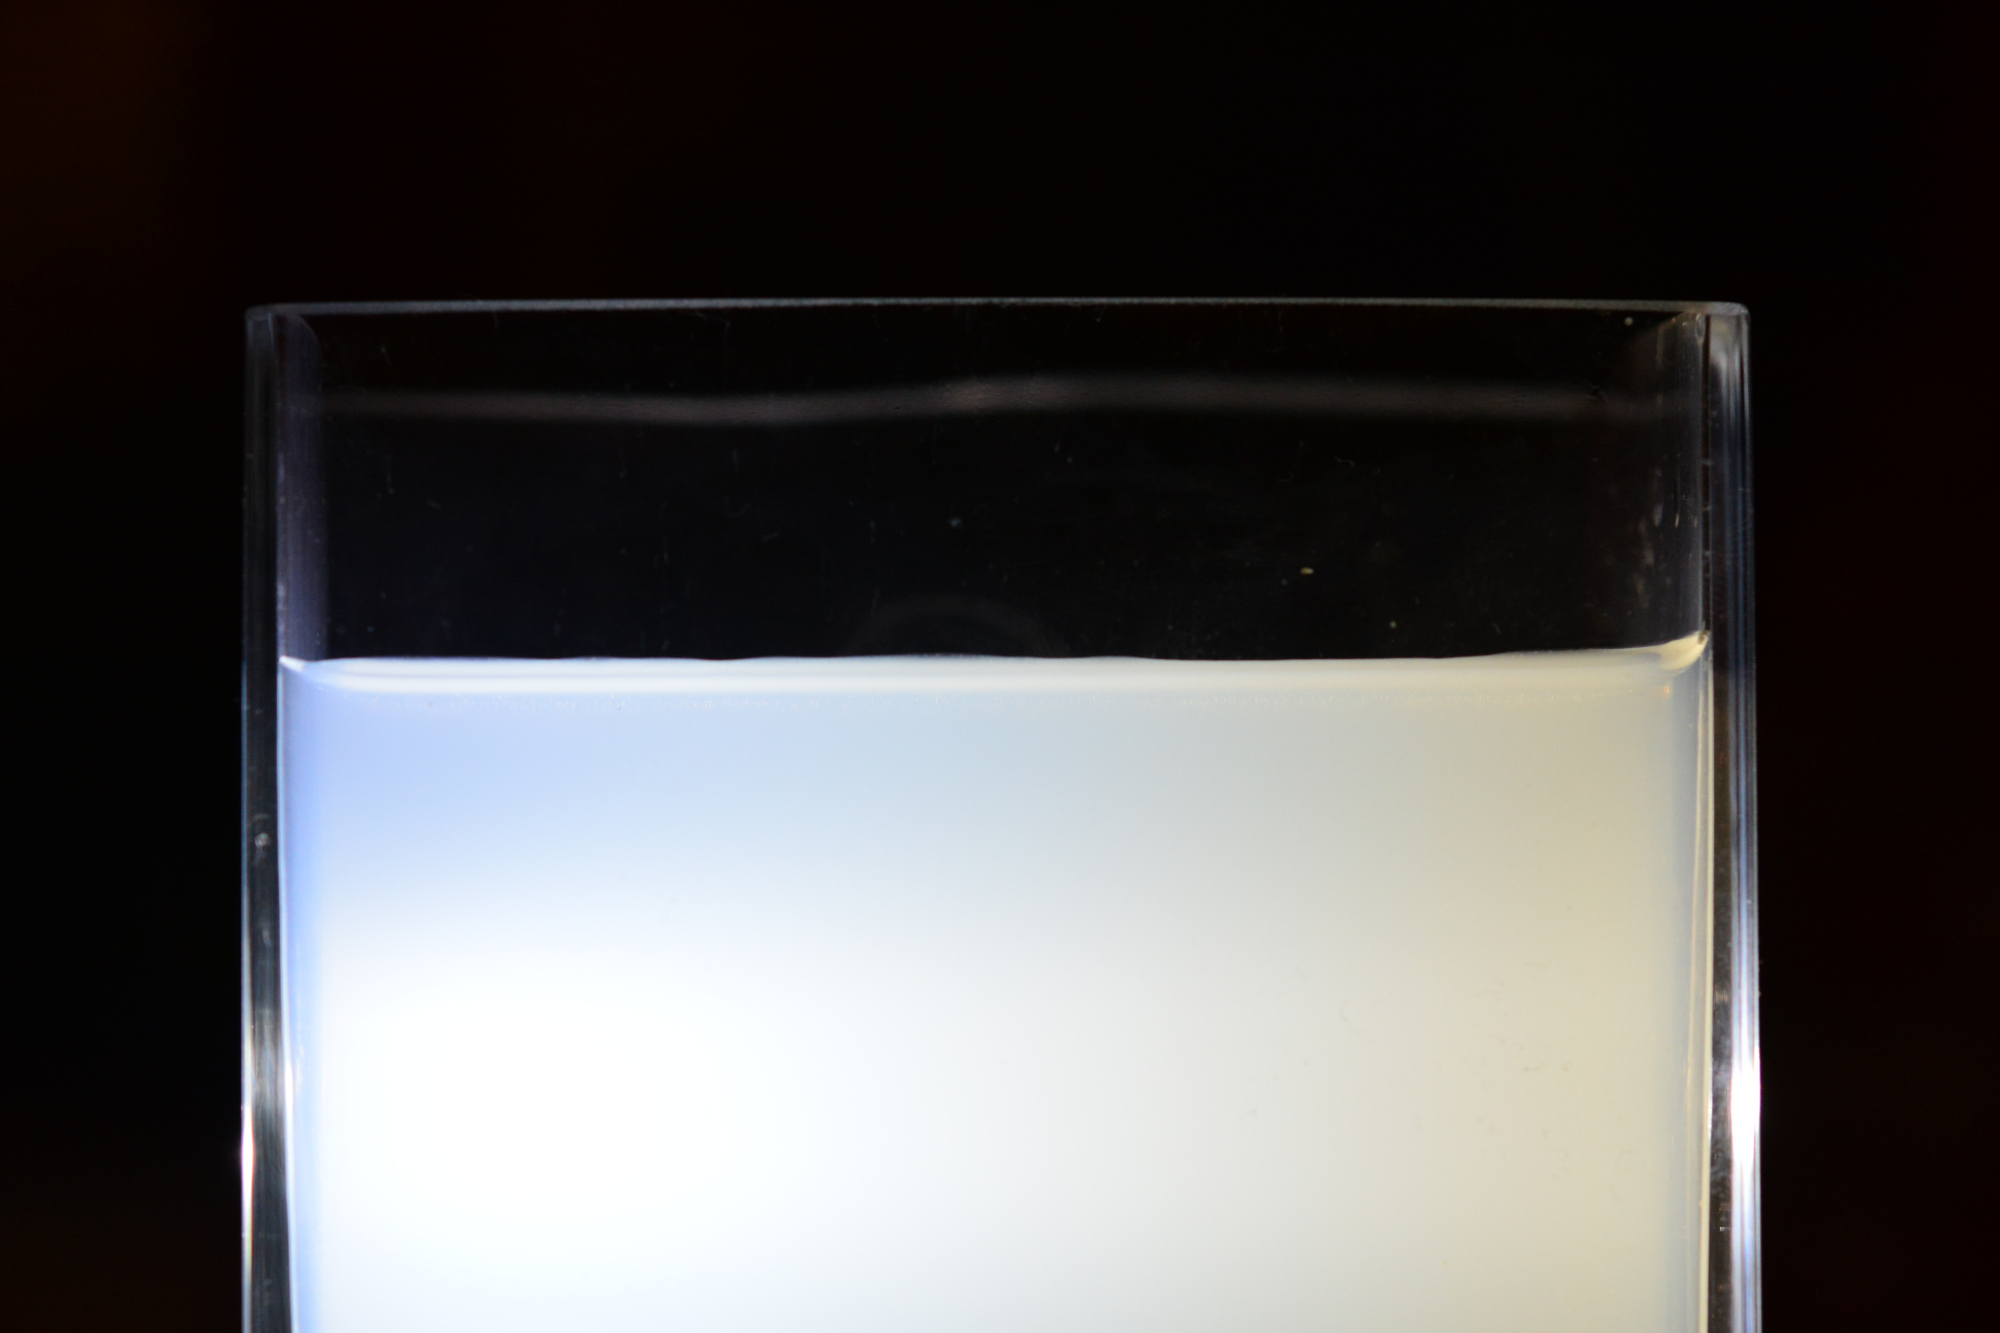
\includegraphics[width=7truecm]{slike/07_mleko.jpg}\hfill
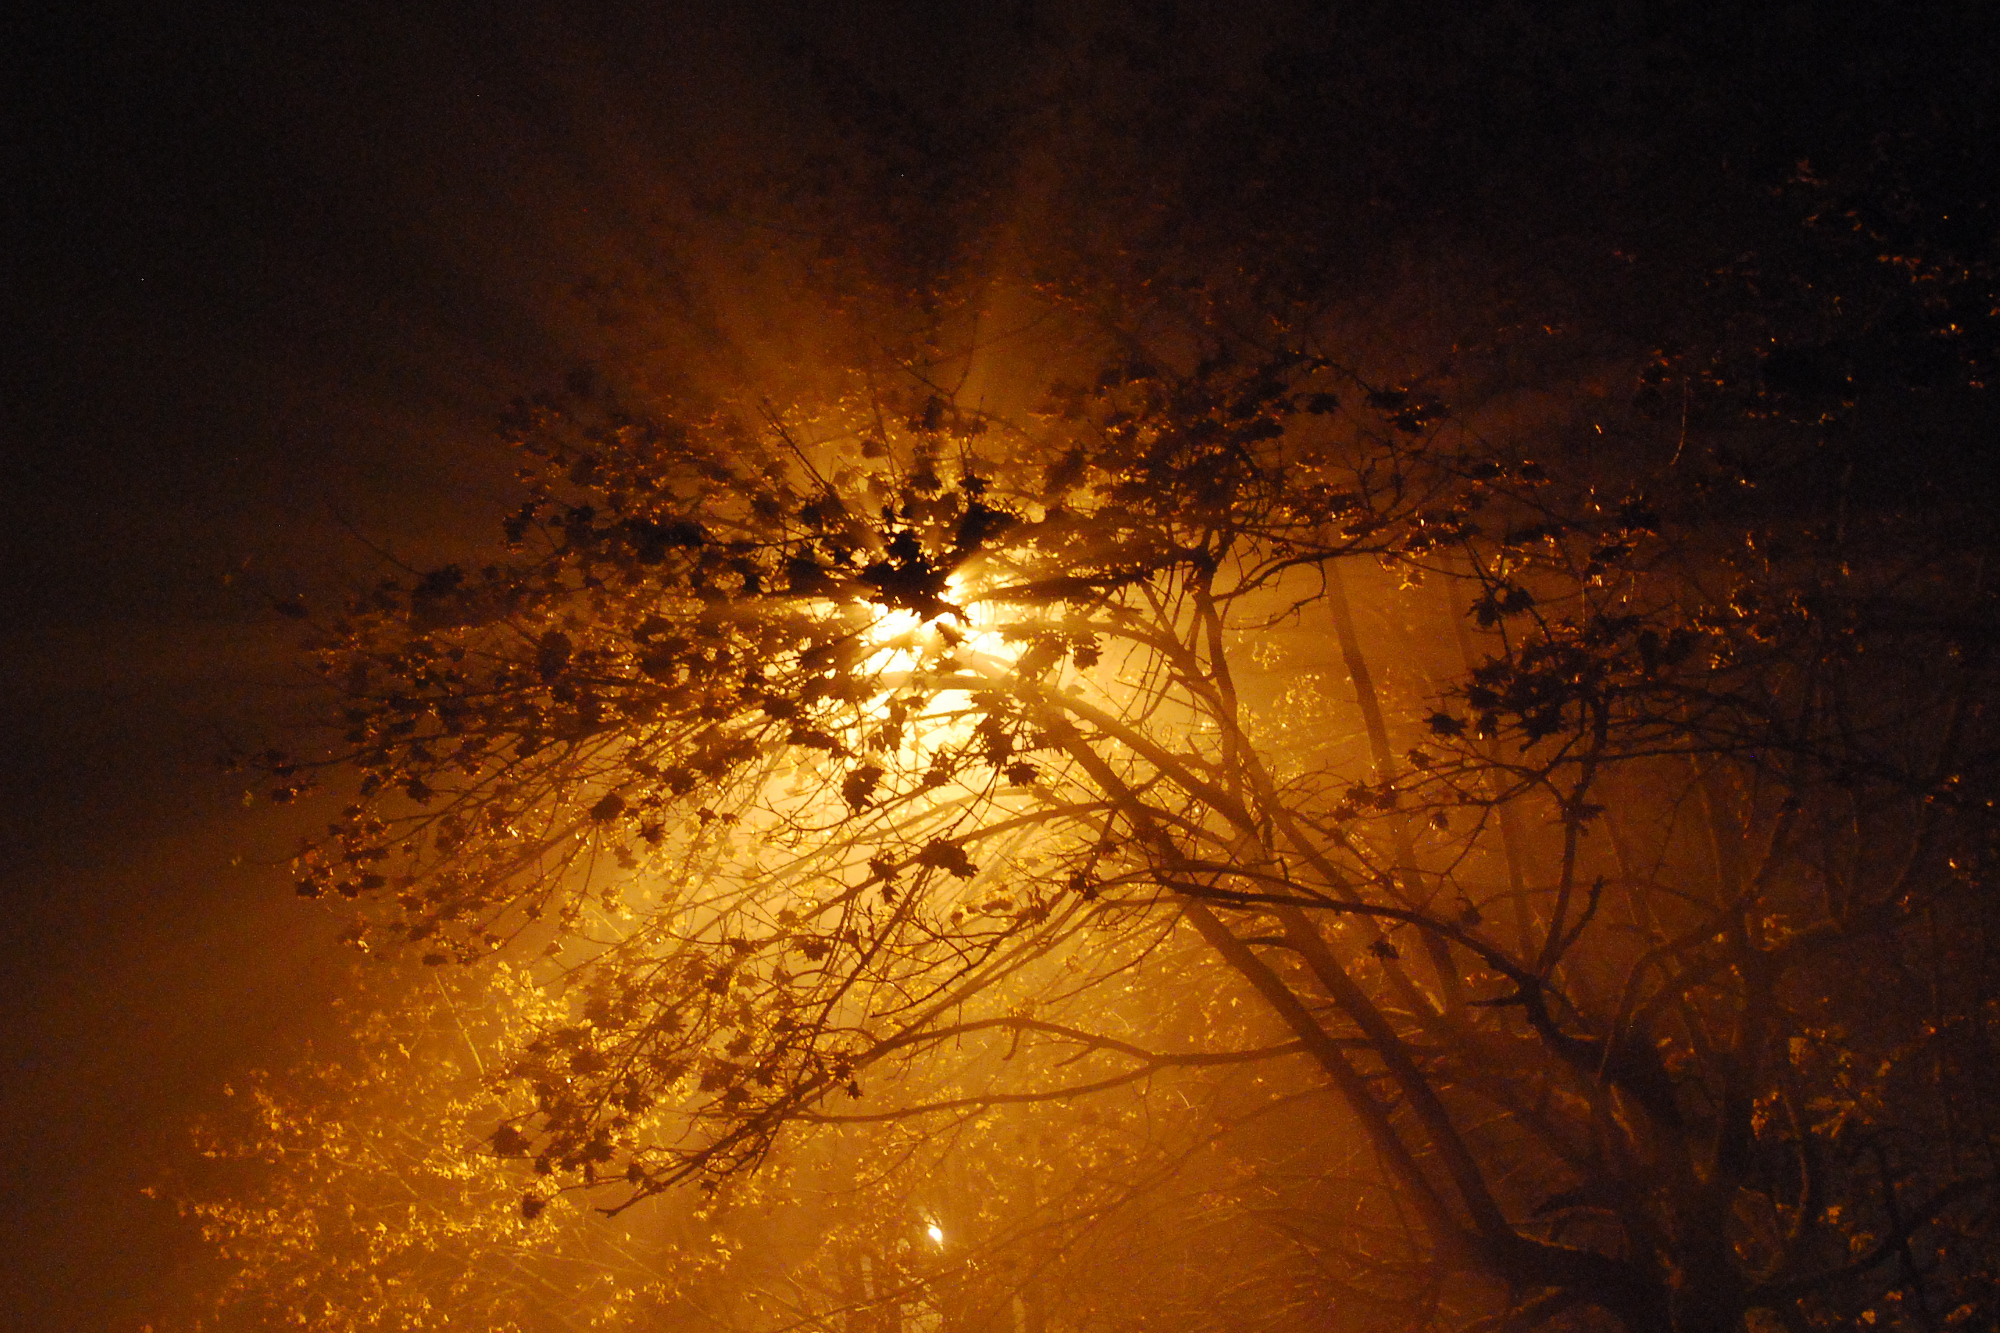
\includegraphics[width=7truecm]{slike/07_megla.jpg}
\caption{Sipanje svetlobe v mešanici vode in mleka (levo) ter sipanje svetlobe 
cestne svetilke v megli (desno).}
\label{fig:07_Sipanje}
\end{figure}

Ko elektromagnetno valovanje vpade na majhen delec, izmenično električno 
polje deluje na njegov naboj in ga periodično izmika iz ravnovesne lege. 
Nastali oscilirajoči električni dipol 
podobno kot antena oddaja (seva) elektromagnetno valovanje. V velikih 
homogenih območjih se prispevki vseh atomov izpovprečijo in svetloba
se širi zgolj v vpadni smeri. Kadar pa je območje nehomogeno, se 
prispevki posameznih atomov med seboj razlikujejo in svetloba se širi 
tudi v smereh, ki se razlikujejo od vpadne smeri. Pravimo, da se svetloba siplje. 
Zaradi sipanja svetlobe se gostota svetlobnega toka v smeri vpadnega valovanja
zmanjšuje, kar imenujemo slabljenje, atenuacija ali ekstinkcija. Podobno učinkuje tudi 
absorpcija svetlobe v snovi, zato je celotno slabljenje sestavljeno iz 
prispevkov sipanja in absorpcije (slika~\ref{fig:07_skica}\,a). Pri obravnavni sipanja se bomo omejili na 
dielektrične snovi, ki svetlobe ne absorbirajo. Sipanje, pri katerem se 
svetloba ne absorbira in energija ne izgublja, imenujemo elastično sipanje.\index{Sipanje!{elastično}}

\begin{figure}[!ht]
\centering
\def\svgwidth{100truemm} 
\input{slike/07_skica01.pdf_tex}
\caption{Zaradi sipanja in absorpcije se intenziteta svetlobe, ki potuje skozi 
nehomogeno snov, zmanjšuje (a). Zmanjševanje svetlobnega toka $P$ in 
gostote svetlobnega toka $j$ izpeljemo z zapisom
zmanjševanja v tanki plasti snovi debeline $\Delta z$ (b).}
\label{fig:07_skica}
\vglue-2truemm
\end{figure}

Naj svetloba z gostoto svetlobnega toka $j$ vpada na tanko plast snovi 
vzdolž smeri $z$ (slika~\ref{fig:07_skica}\,b). Prostornina osvetljenega 
dela naj bo $V = S \Delta z$,
v njem pa naj bo $N$ sipalcev, to je delcev, na katerih se svetloba siplje. 
Vsak od sipalcev prispeva k zmanjšanju svetlobnega toka:
\begin{equation}
\Delta P_1 = - \sigma_S j.
\label{eq:07_01}
\end{equation}
pri čemer vpeljemo sipalni presek $\sigma_S$\index{Sipalni presek} kot razmerje med svetlobnim 
tokom sipane svetlobe in gostoto svetlobnega toka vpadne svetlobe. 
Sipalni presek ima enoto ploščine, vendar se razlikuje od prečnega preseka sipalca.
Njegova velikost je določena s tem, kako močno sipalec vpliva na vpadno 
svetlobo: delci z večjim sipalnim presekom bolj sipljejo svetlobo in obratno, 
delci z manjšim sipalnim presekom manj zmotijo potek vpadnega valovanja. 
Sipalni presek je specifičen za izbrano snov, je pa odvisen od valovne 
dolžine valovanja, ki vpada na delec. 

Skupni prispevek vseh delcev v osvetljenem delu snovi k zmanjšanju svetlobnega toka
je:
\begin{equation}
\Delta P = - N \sigma_S j.
\label{eq:07_02}
\end{equation}
Vpeljemo gostoto sipalcev $\varrho = N/V$ in dobimo:
\begin{equation}
\Delta P = - \sigma_S j\,\varrho S \Delta z.
\label{eq:07_03}
\end{equation}
Izraz delimo s presekom snopa $S$ in ga zapišemo v diferencialni obliki:
\begin{equation}
dj = \frac{dP}{S} = - \sigma_S j\, \varrho dz.
\label{eq:07_04}
\end{equation}
Vpeljemo $\mu = \sigma_S \varrho$ kot koeficient slabljenja\index{Koeficient slabljenja}
(tudi atenuacijski ali ekstinkcijski\index{Atenuacijski koeficient|see{Koeficient slabljenja}}
\index{Ekstinkcijski koeficient|see{Koeficient slabljenja}}
koeficient). Sorazmeren je z gostoto delcev, na katerih se svetloba siplje, sorazmernostni
faktor pa je sipalni presek. Enačbo~(\ref{eq:07_04}) integriramo in dobimo:
\boxeq{eq:BL}{
j(z) = j_0 e^{-\mu z},
}
pri čemer je $j_0$ gostota vpadnega svetlobnega toka. Zapisana enačba 
opisuje eksponentno pojemanje intenzitete vpadne svetlobe zaradi 
sipanja in je povsem analogna Beer-Lambertovem zakon za absorpcijo svetlobe v snovi. 

\begin{remark}
Poleg totalnega sipalnega preseka $\sigma_S$, ki pove, kako močno se svetloba siplje,
pogosto vpeljemo tudi diferencialni sipalni presek:\index{Sipalni presek!totalni}
\begin{equation}
\frac{d\sigma}{d\Omega} = \frac{j(\vartheta)}{j_0} r^2,
\label{eq:07_04a}
\end{equation}
pri čemer je $r$ razdalja od sipalca do opazovalca, kot $\vartheta$ pa merimo
glede na smer vpadne svetlobe. Diferencialni sipalni\index{Sipalni presek!diferencialni}
presek pove, kako močno se svetloba siplje v prostorski kot $d\Omega$ pri kotu $\vartheta$. 
Integral diferencialnega sipalnega preseka po prostorskem kotu da totalni
sipalni presek:
\begin{equation}
\sigma_S = \int \frac{d\sigma}{d\Omega} d\Omega.
\label{eq:07_04b}
\end{equation}
\end{remark}

\section{Sipanje na vezanem elektronu in Rayleighovo sipanje}\index{Sipanje!{Rayleighovo}}
Najprej si podrobneje oglejmo sipanje na delcih, ki so bistveno manjši 
od valovne dolžine svetlobe (npr. atomi in molekule). Za njih velja $R \ll \lambda$, 
pri čemer je $R$ značilna dimenzija delca. Tako sipanje imenujemo 
Rayleighovo sipanje po angleškemu fiziku Lordu 
Rayleighu (1842--1919).\index{Rayleighovo sipanje}\index{Rayleigh, Lord}

Uporabimo Lorentzev model atoma, ki smo ga spoznali v razdelku~\ref{chap:lomni}.
V njem elektron opišemo kot lahko kroglico z maso $m$ in nabojem $e$, ki je z vzmetjo\index{Lorentzev model!sipanje} 
s koeficientom $k_0$ vezana na bistveno večje jedro. Ko
na atom vpade elektromagnetno valovanje, deluje na elektron 
Lorentzeva sila in elektron zaniha. Naj svetloba na atom vpada vzdolž 
smeri $x$, njena polarizacija pa naj bo vzporedna osi $z$ 
(glej sliko~\ref{fig:07_koor2}).\footnote{Zaradi uveljavljenega koordinatnega sistema
pri kasnejšem zapisu sevajočega dipola smo pri tem računu zasukali koordinatni sistem.}
\begin{figure}[!ht]
\centering
\def\svgwidth{90truemm} 
\input{slike/07_koor2.pdf_tex}
\caption{Vpadna svetloba, ki se širi vzdolž osi $x$, naj bo polarizirana vzdolž
osi $z$, sipana svetloba pa naj se širi pod kotom $\vartheta$ glede na os $z$. Vektor 
$\mathbf{p}$ (zelena) označuje dipol, ki se inducira pod vplivom vpadnega električnega 
polja.}
\label{fig:07_koor2}
\vglue-3truemm
\end{figure}

Newtonov zakon za gibanje elektrona smo na splošno zapisali z enačbo~(\ref{eq:09_02}), 
zdaj pa dušenje zanemarimo in poenostavljeno zapišemo:
\begin{equation}
m \ddot{z} + k_0 z = e E = e E_0 e^{-i\omega t},
\label{eq:07_50}
\end{equation}
pri čemer smo vpadno polje $E$ zapisali kot ravno valovanje s frekvenco $\omega$ v
izhodišču pri $x=0$. 
Uporabimo nastavek za periodično spreminjanje lege, pri čemer ima vsiljeno 
nihanje elektrona enako smer in enako frekvenco kot vpadno valovanje. Dobimo resonančno odvisnost:
\begin{equation}
z = \frac{e/m}{\omega_0^2-\omega^2}E,
\label{eq:07_51}
\end{equation}
pri čemer je $\omega_0 = \sqrt{k_0/m}$ lastna frekvenca nihanja.
Inducirani dipolni moment, ki nastane zaradi premikanja elektrona, 
je enak:
\begin{equation}
p = ez  = \frac{e^2/m}{\omega_0^2-\omega^2} E = 
\frac{e^2/m}{\omega_0^2-\omega^2}E_0 e^{-i\omega t}.
\label{eq:07_52}
\end{equation}
S tem smo pokazali, da dipolni moment, ki se inducira v atomu, niha s frekvenco, 
ki je enaka frekvenci vpadnega valovanja, njegova amplituda pa je funkcija te frekvence.

Za nihajoči dipolni moment vemo, da oddaja elektromagnetno valovanje -- seva. 
Sevalno polje v velikih oddaljenostih od električnega dipola zapišemo 
kot:\footnote{Glej npr. Strnad, {\it Fizika, drugi del}, DMFA-založništvo (2018) in
Podgornik in Vilfan, {\it Elektromagnetno polje}, DMFA-založništvo (2012).}
\begin{equation}
\mathbf{E}_\mathrm{sev} = \frac{1}{4 \pi \varepsilon_0 c^2 r}
\left(\ddot{\mathbf{p}} \times \frac{\mathbf{r}}{r}\right)\times \frac{\mathbf{r}}{r}.
\label{eq:07_12}
\end{equation}
Vstavimo sinusno nihajoč električni dipol (enačba~\ref{eq:07_52})
in izračunamo vektorski produkt, pri čemer upoštevamo, da je smer induciranega
dipola vzdolž osi $z$. Za sevalno polje dobimo:\index{Sevalno polje dipola}
\begin{equation}
\mathbf{E}_\mathrm{sev} = -
\frac{e^2}{4 \pi \varepsilon_0\,m c^2}\frac{\omega^2}{\omega_0^2-\omega^2}E_0
\sin \vartheta \left(\frac{e^{ikr - i\omega t}}{r}\right) \hat{\mathbf{e}}_\vartheta.
\label{eq:dipolE}
\end{equation}
V velikih oddaljenostih od dipola je smer jakosti električnega polja vzdolž smeri enotskega
vektorja $\hat{\mathbf{e}}_\vartheta$. V tem približku se amplituda polja zmanjšuje 
kot $1/r$. Vzdolž smeri $z$, to je vzdolž smeri polarizacije vpadnega valovanja, 
je jakost izsevanega električnega polja enaka nič.\index{Jakost električnega polja}

Podobno kot jakost električnega polja izračunamo tudi jakost magnetnega polja:
\begin{equation}
\mathbf{H}_\mathrm{sev} = \frac{1}{4 \pi c r}
\left(\ddot{\mathbf{p}} \times \frac{\mathbf{r}}{r}\right) = - \frac{e^2}{4 \pi m c}
\frac{\omega^2}{\omega_0^2-\omega^2}E_0\sin \vartheta
\left(\frac{e^{ikr - i\omega t}}{r}\right) \hat{\mathbf{e}}_\varphi.
\label{eq:dipolH}
\end{equation}
Jakost izsevanega magnetnega polja je pravokotna na smer dipola in 
hkrati tudi na smer jakosti električnega polja. Podobno kot jakost
električnega polja tudi jakost magnetnega polja pojema z oddaljenostjo
od dipola kot $1/r$ in je enaka nič vzdolž smeri $z$.

Gostoto energijskega toka sevalnega polja izračunamo kot povprečje\index{Sipanje!{kotna odvisnost}}
Poyntingovega vektorja (enačba~\ref{eq:Poyntingov}):\index{Poyntingov vektor}
\boxeq{eq:dipolj}{
\mathbf{j}_\mathrm{sev} = \langle \mathbf{E}_\mathrm{sev}
\times \mathbf{H}_\mathrm{sev}  \rangle 
= \frac{e^4}{32 \pi^2 \varepsilon_0\,m^2 c^3}\frac{1}{r^2}
\left(\frac{\omega^2}{\omega_0^2-\omega^2}\right)^2
E_0^2 \sin^2 \vartheta \,\mathbf{e}_r.
}
Smer gostote svetlobnega toka je radialno navzven, 
kar pomeni, da se zaradi sevanja vpadni energijski tok preusmeri iz vpadne smeri
v druge smeri. Posledično intenziteta svetlobe v vpadni smeri slabi, v ostalih smereh pa se 
pojavi sipana svetloba. Gostota svetlobnega toka 
pojema obratno sorazmerno s kvadratom oddaljenosti od izhodišča, kar je v skladu
z ohranitvijo energije.  
Sevalno polje je močno odvisno od kota $\vartheta$: vzdolž smeri vpadne 
polarizacije (os $z$) sipanja ni, največje sipanje pa je v smeri pravokotno glede na smer 
polarizacije vpadne svetlobe ($\vartheta = 90\si{\degree}$). Porazdelitev sipane svetlobe 
je osno simetrična okoli osi $z$, njena odvisnost v ravnini $xz$ pa je prikazana na 
sliki~\ref{fig:07_dipol}. Zanimivo je, da se enako svetlobe siplje v smeri naprej kot nazaj.
\begin{figure}[!ht]
\centering
\def\svgwidth{60truemm} 
\input{slike/07_dipol.pdf_tex}
\caption{Intenziteta sipane svetlobe je močno odvisna od smeri: v smeri induciranega
dipola (zelena puščica) je enaka nič, največja pa je v ravnini, ki je pravokotna na dipol. }
\label{fig:07_dipol}
\end{figure}

Poleg kotne odvisnosti ima gostota svetlobnega toka, ki jo izseva 
inducirani dipol,\index{Sipanje!{frekvenčna odvisnost}} 
tudi zelo pomembno frekvenčno odvisnost. Omejimo se na vpadno valovanje, katerega 
frekvenca je daleč od resonančnih frekvenc atoma in za katero velja 
$\omega \ll \omega_0$. Takrat lahko v imenovalcu enačbe~(\ref{eq:dipolj}) 
frekvenco $\omega$ zanemarimo, v števcu
pa jo seveda ohranimo. Vpeljemo $j_0$ kot gostoto vpadnega energijskega toka in dobimo:
\begin{equation}
j_\mathrm{sev}
= j_0 \frac{e^4}{16 \pi^2 \varepsilon_0^2 m^2 c^4 \omega_0^4} \frac{\omega^4}{r^2} 
\sin^2 \vartheta.
\label{eq:07_53}
\end{equation}
Za Rayleighovo sipanje je značilna četrta potenca v odvisnosti od frekvence 
vpadne svetlobe:
\boxeq{eq:rayleigh}{
j_\mathrm{sev} \propto \omega^4 \propto \frac{1}{\lambda^4}.
}
Valovanja s večjimi frekvencami (in krajšimi valovnimi dolžinami) se tako 
bistveno bolj sipljejo kot valovanja z daljšimi valovnimi dolžinami 
(slika~\ref{fig:07_rayleighlambda}). Kadar se
siplje vidna bela svetloba, se modri del spektra siplje bistveno močneje kot rdeči
del. To ima zelo pomembno -- in vidno -- posledico.
\begin{figure}[!ht]
\vglue-2truemm
\centering
\def\svgwidth{60truemm} 
\input{slike/07_rayleighlambda.pdf_tex}
\caption{Relativna intenziteta sipane svetlobe v odvisnosti od valovne dolžine vpadnega
valovanja. Modri del spektra se siplje bistveno močneje od rdečega dela spektra.}
\label{fig:07_rayleighlambda}
\vglue-9truemm
\end{figure}

\begin{remark}
Pri zapisu Rayleighovega sipanja smo privzeli, da je $\omega \ll \omega_0$. Ta zapis
velja za elastično vezan elektron. V nasprotnem primeru, ko je $\omega \gg \omega_0$, 
govorimo o Thomsonovem sipanju, ki opisuje elastično sipanje elektromagnetnega valovanja 
na prostem elektronu. Pri tem pogoju se v enačbi~(\ref{eq:dipolj}) frekvenčna 
odvisnost okrajša in za Thomsonovo sipanje je značilno, da je intenziteta\index{Thomsonovo 
sipanje}\index{Sipanje!{Thomsonovo}}
sipane svetlobe neodvisna od frekvence vpadnega valovanja. 
Medtem ko Rayleighovo sipanje tipično opazujemo z vidno
svetlobo, Thomsonovo sipanje navadno opazujemo z rentgenskimi žarki.
\end{remark}

Izraz za intenziteto sipane svetlobe (enačba~\ref{eq:07_53}) lahko še malo 
preoblikujemo. Zapišemo dipolni moment $p$ kot produkt naboja $e$ in odmika 
iz ravnovesne lege $eE/k$. Izrazimo še $k$ z lastno krožno frekvenco in dobimo:
\begin{equation}
p = \frac{e^2 E}{m\omega_0^2}.
\label{eq:07_54}
\end{equation}
Sledi:
\boxeq{eq:07_55}{
\mathbf{j}_\mathrm{sev}
= \frac{p^2}{32 \pi^2 \varepsilon_0 c^3} \frac{\omega^4}{r^2} 
\sin^2 \vartheta \,\mathbf{e}_r.
}
Z vpeljavo dipolnega momenta smo izračunani izraz posplošili in njegovo
veljavnost razširili na večje delce, v katerih se ob vpadu elektromagnetnega 
valovanja inducira električni dipol.

\begin{example}{\bf Sipanje na majhnih dielektričnih kroglicah.}\index{Sipanje!{na kroglicah}}
Obravnavajmo sipanje svetlobe na dielektričnih kroglicah z
dielektričnostjo $\varepsilon_2$, dielektričnost 
okolice pa naj bo enaka $\varepsilon_1$. Kroglice naj bodo majhne ($R < \lambda$),
zato da lahko privzamemo, da je električno polje 
vpadnega valovanja $E$ znotraj celotnega delca enako. 

Inducirani dipolni moment v kroglici izračunamo iz 
elektrostatike z upoštevanjem robnih pogojev na površini 
kroglice\footnote{Glej npr. Stratton, {\it Electromagnetic Theory}, različne izdaje.}
in ga zapišemo kot:
\begin{equation}
p = 4 \pi \varepsilon_0 R^3 \,\frac{\varepsilon-1}{\varepsilon +2} E,
\label{eq:07_56}
\end{equation}
pri čemer je $\varepsilon = \varepsilon_2/\varepsilon_1$. 

Do povsem enakega rezultata pridemo tudi z upoštevanjem zveze med polarizirnostjo in 
dielektričnostjo snovi (enačba~\ref{eq:09_35a}), kjer zapišemo:
\begin{equation}
p = \alpha E = \frac{3\varepsilon_0}{\varrho}\frac{\varepsilon-1}{\varepsilon+2}E,
\label{eq:07_57}
\end{equation}
pri čemer je $\varrho$ gostota delcev. Inverz gostote je prostornina, ki pripada
enemu delcu, to je $4\pi R^3/3$. Ko vstavimo prostornino enega delca, dobimo enačbo~(\ref{eq:07_56}).

Oba izraza dokazujeta, da se svetloba siplje le, če sta dielektričnosti 
kroglice in okoliške snovi različni.
Od razlike lomnih količnikov je odvisna intenziteta sipane svetlobe, medtem ko
kotna odvisnost in odvisnost od valovne dolžine ostajata nespremenjeni.
\end{example}

Vrnimo se k izrazu za gostoto energijskega toka sipane 
svetlobe (enačba~\ref{eq:07_55}) in upoštevajmo velikost induciranega 
dipolnega momenta v dielektrični kroglici (enačba~\ref{eq:07_56}). Na danem
mestu je gostota svetlobnega toka sipane svetlobe sorazmerna:
\begin{equation}
j_\mathrm{sev} \propto \omega^4 p^2 \propto E^2 \frac{R^6}{\lambda^4}.
\label{eq:07_17}
\end{equation}
Sipalni presek, ki ga izračunamo kot razmerje med sipanim svetlobnim tokom in\index{Sipalni presek}
vpadno gostoto svetlobnega toka, je sorazmeren s šesto potenco polmera 
delca in obratno sorazmeren s četrto potenco valovne dolžine svetlobe.

\begin{example}{\bf Zakaj je nebo modro?}\index{Modro nebo}\index{Sonce}
Preden svetloba s Sonca doseže Zemljino površje, prepotuje Zemljino atmosfero.
Pri tem se del svetlobe absorbira (najizrazitejše so absorpcije v ultravijoličnem delu 
spektra na ozonski plasti ter v infrardečem spektru na molekulah vode in ogljikovega 
dioksida). Preostala svetloba potuje skozi atmosfero in se pri tem na molekulah
Rayleighovo siplje. Zaradi močne odvisnosti intenzitete sipanja od valovne dolžine 
svetlobe (enačba~\ref{eq:rayleigh}) se modri odtenki sipljejo 
bistveno bolj kot svetloba rdečih odtenkov z daljšo valovno dolžino.
Na primer: svetloba z $\lambda = 400~\si{\nm}$ se siplje 10-krat močneje kot 
svetloba z $\lambda = 710~\si{\nm}$. Ko opazujemo nebo, zaznavamo svetlobo, 
ki se na atmosferi siplje. Ker se modri odtenki sipljejo bolj kot rdeči, 
vidimo nebo modro (slika~\ref{fig:07_Modrina}). 
\begin{figure}[!ht]
\centering
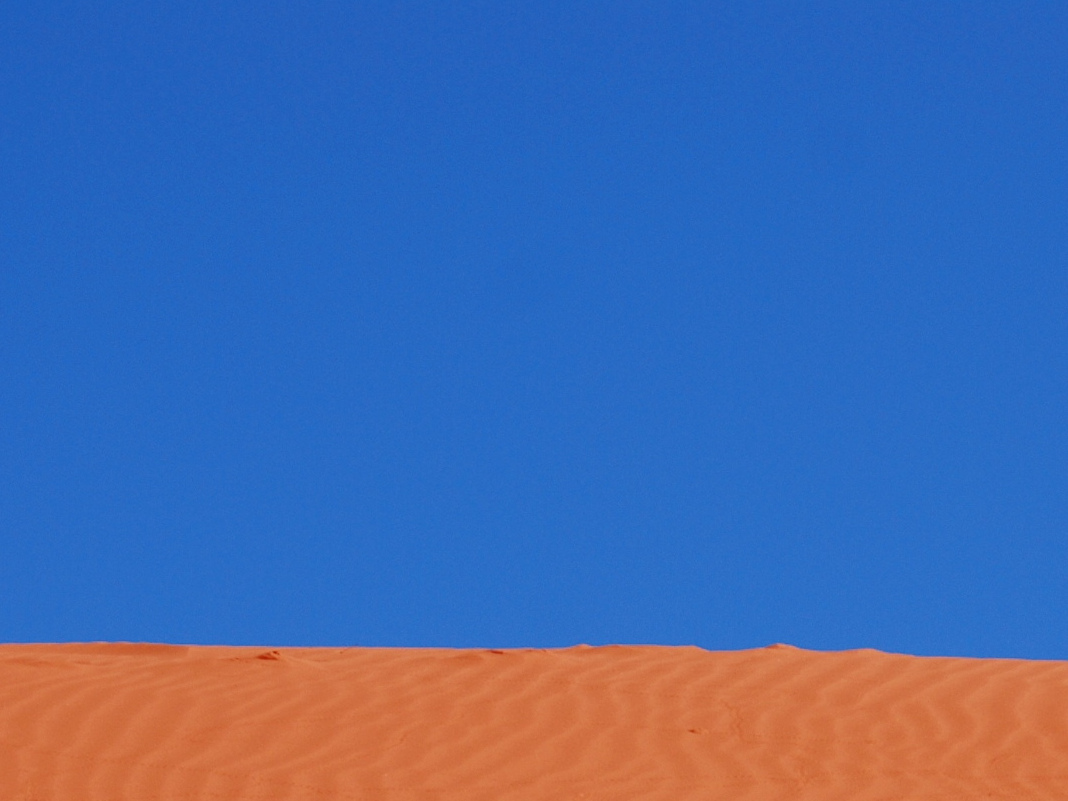
\includegraphics[width=7truecm]{slike/07_ModroNebo.jpg}\hfill
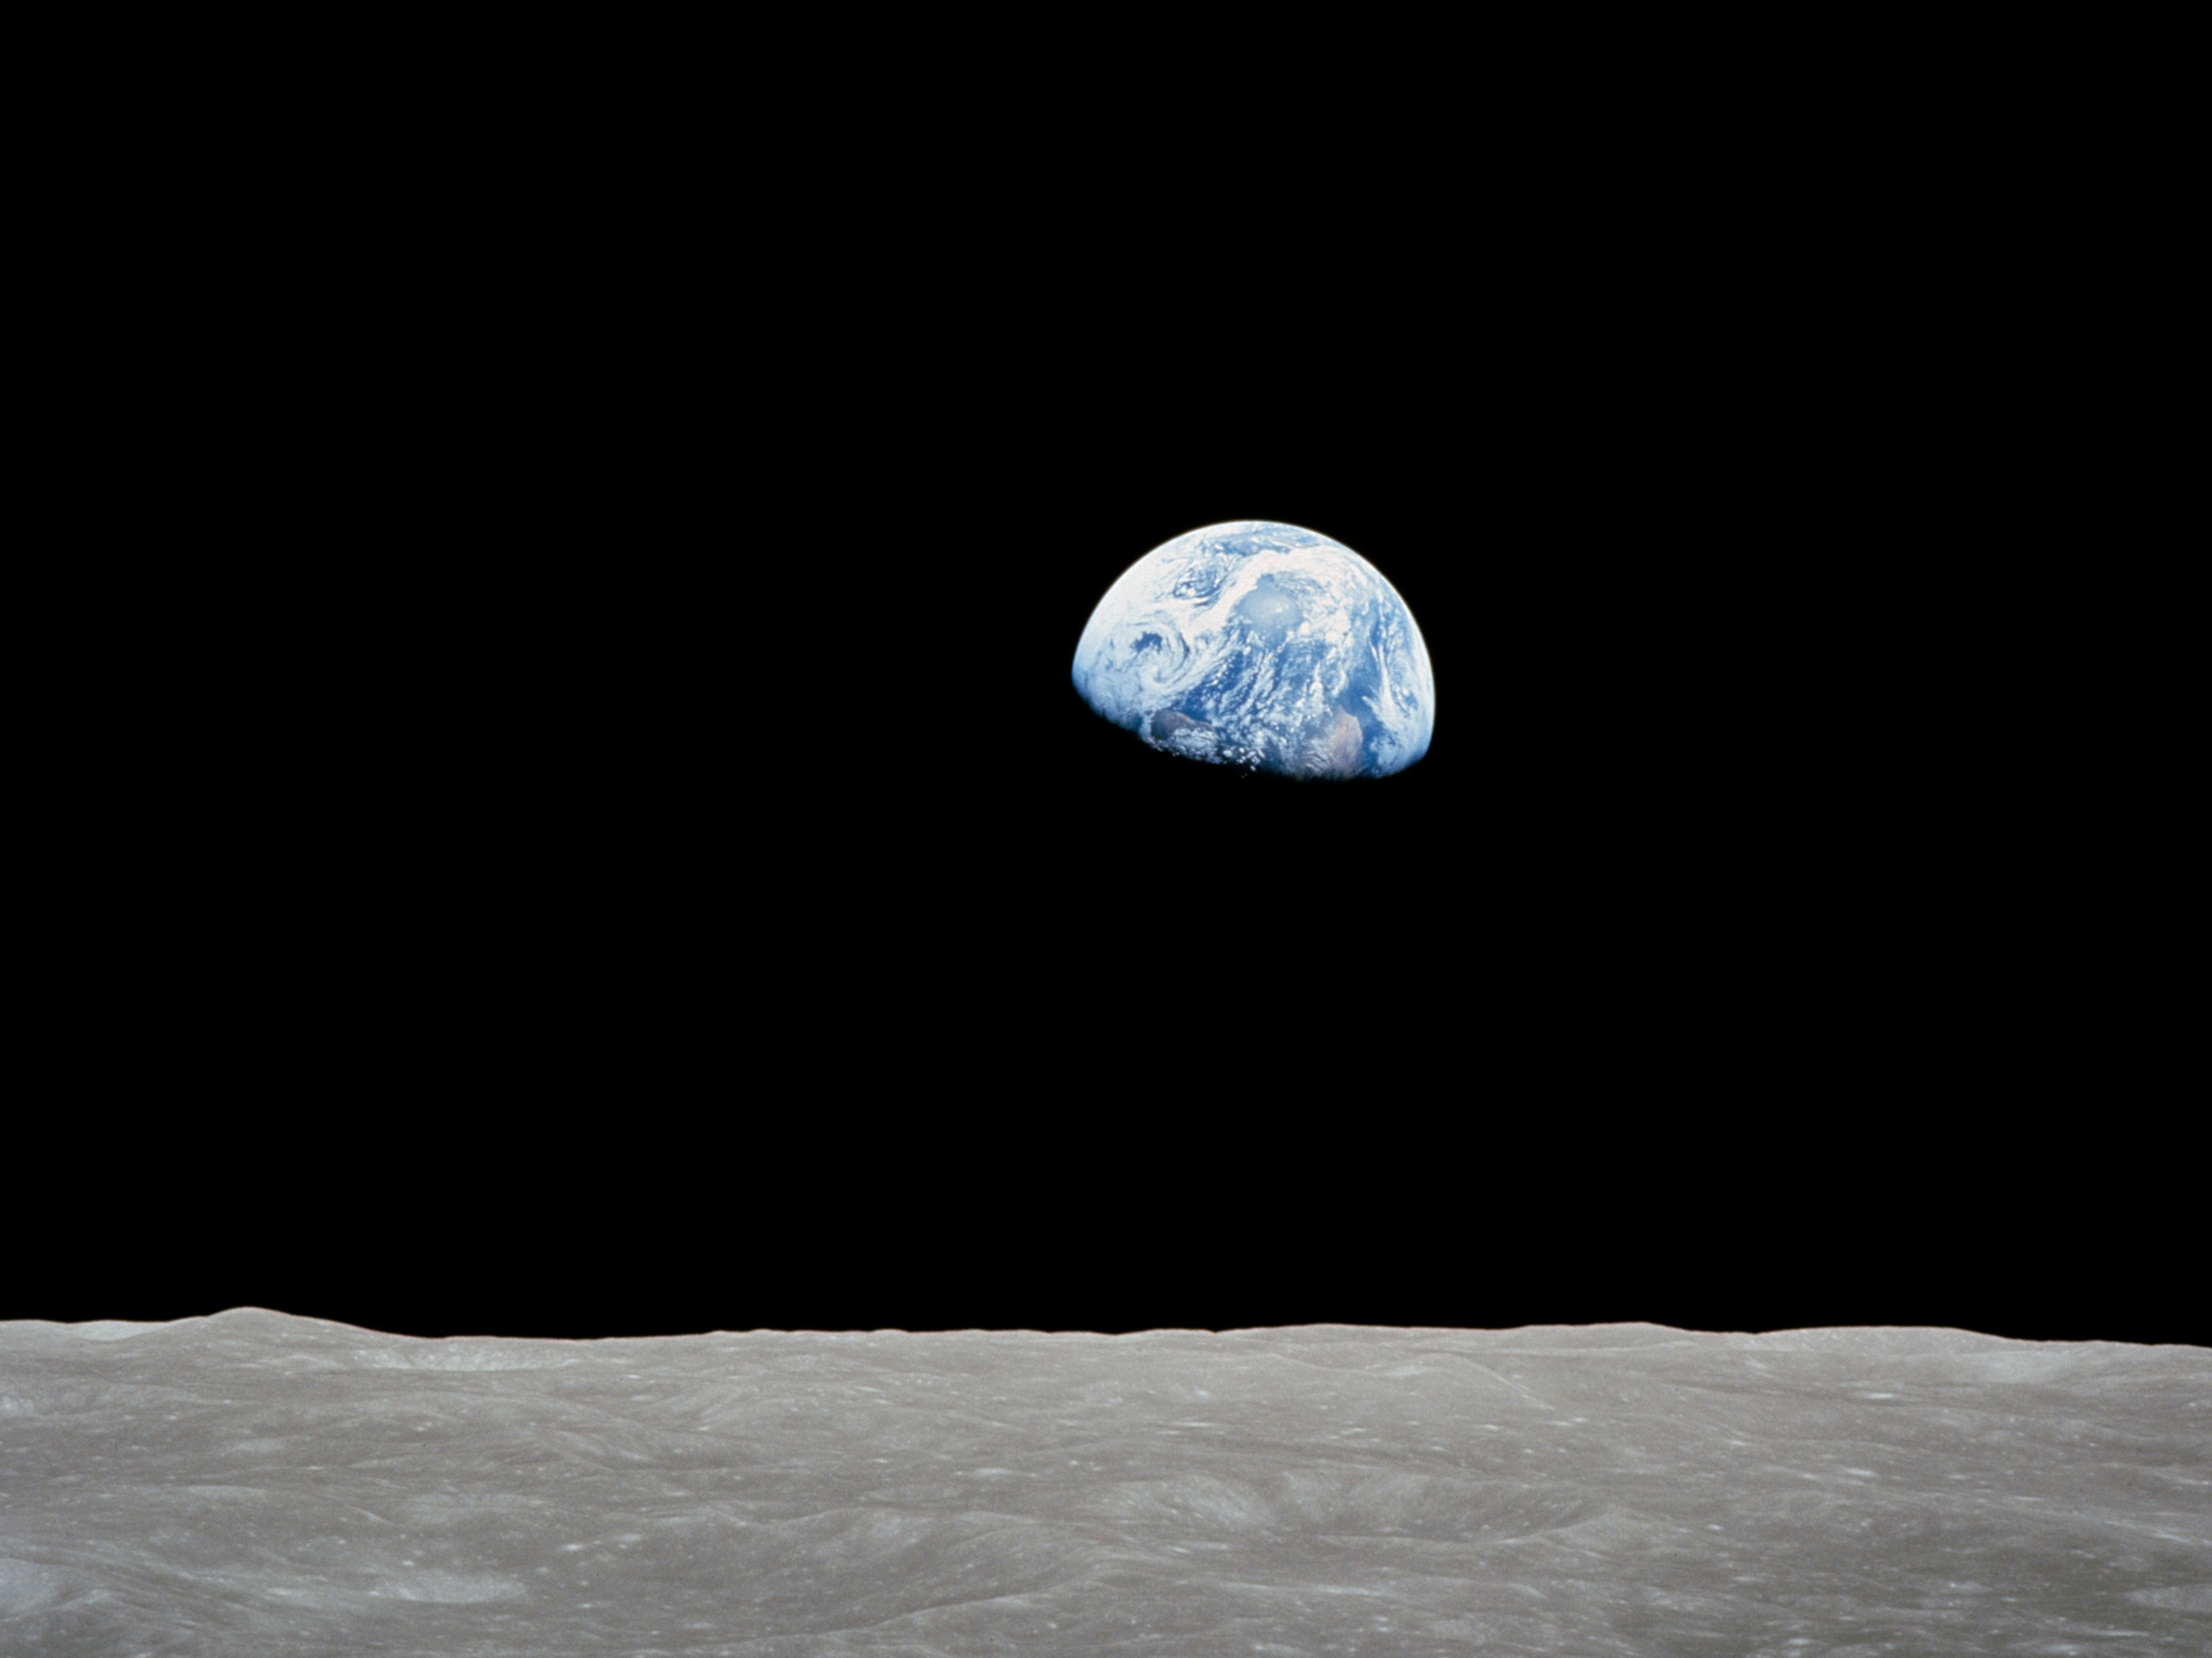
\includegraphics[width=7truecm]{slike/07_Luna.jpg}
\caption{Barva neba je posledica sipanja svetlobe. Ker se močneje siplje 
svetloba s krajšo valovno dolžino, je nebo podnevi videti modro (levo).
Na Luni, kjer ni atmosfere, na kateri bi se svetloba sipala, je nebo 
tudi podnevi povsem črno. Foto z Lune: NASA.}
\label{fig:07_Modrina}
\end{figure}

Seveda se vprašamo, zakaj ne vidimo neba vijoličnega, saj 
ima vijolična svetloba še krajšo valovno dolžino in se zato še močneje siplje. Upoštevati 
moramo spekter sončeve svetlobe, v katerem je vijolična barva manj zastopana od modre, poleg
tega k temu prispeva tudi občutljivost očesa, ki se pri krajših valovnih dolžinah znatno 
zmanjša in vijolične barve ne zaznava tako močno kot modre. 
\end{example}

\begin{example}{\bf In zakaj je sončni zahod rdeč?}\index{Sonce}
Tudi rdeči sončni vzhodi in zahodi so posledica sipanja svetlobe v atmosferi. 
Takrat Sonce leži nizko nad obzorjem in pot svetlobe skozi atmosfero je 
razmeroma dolga. Pogosto je v ozračju bližje površju tudi več vlage, prašnih delcev
in drugih sipalcev. Ker se modra svetloba močno siplje na vse strani, rdeča
pa razmeroma šibko, je večina svetlobe, ki pride do opazovalca iz smeri Sonca,
rdečkaste barve. Zaradi človekove aktivnosti in višjih dnevnih temperatur je 
navadno zvečer v zraku več sipalcev kot proti jutru. Sončni zahodi so zato pogosto
bolj izrazito rdečkasti kot sončni vzhodi (slika~\ref{fig:07_Rdeca}, levo).
\end{example}
\begin{figure}[!ht]
\centering
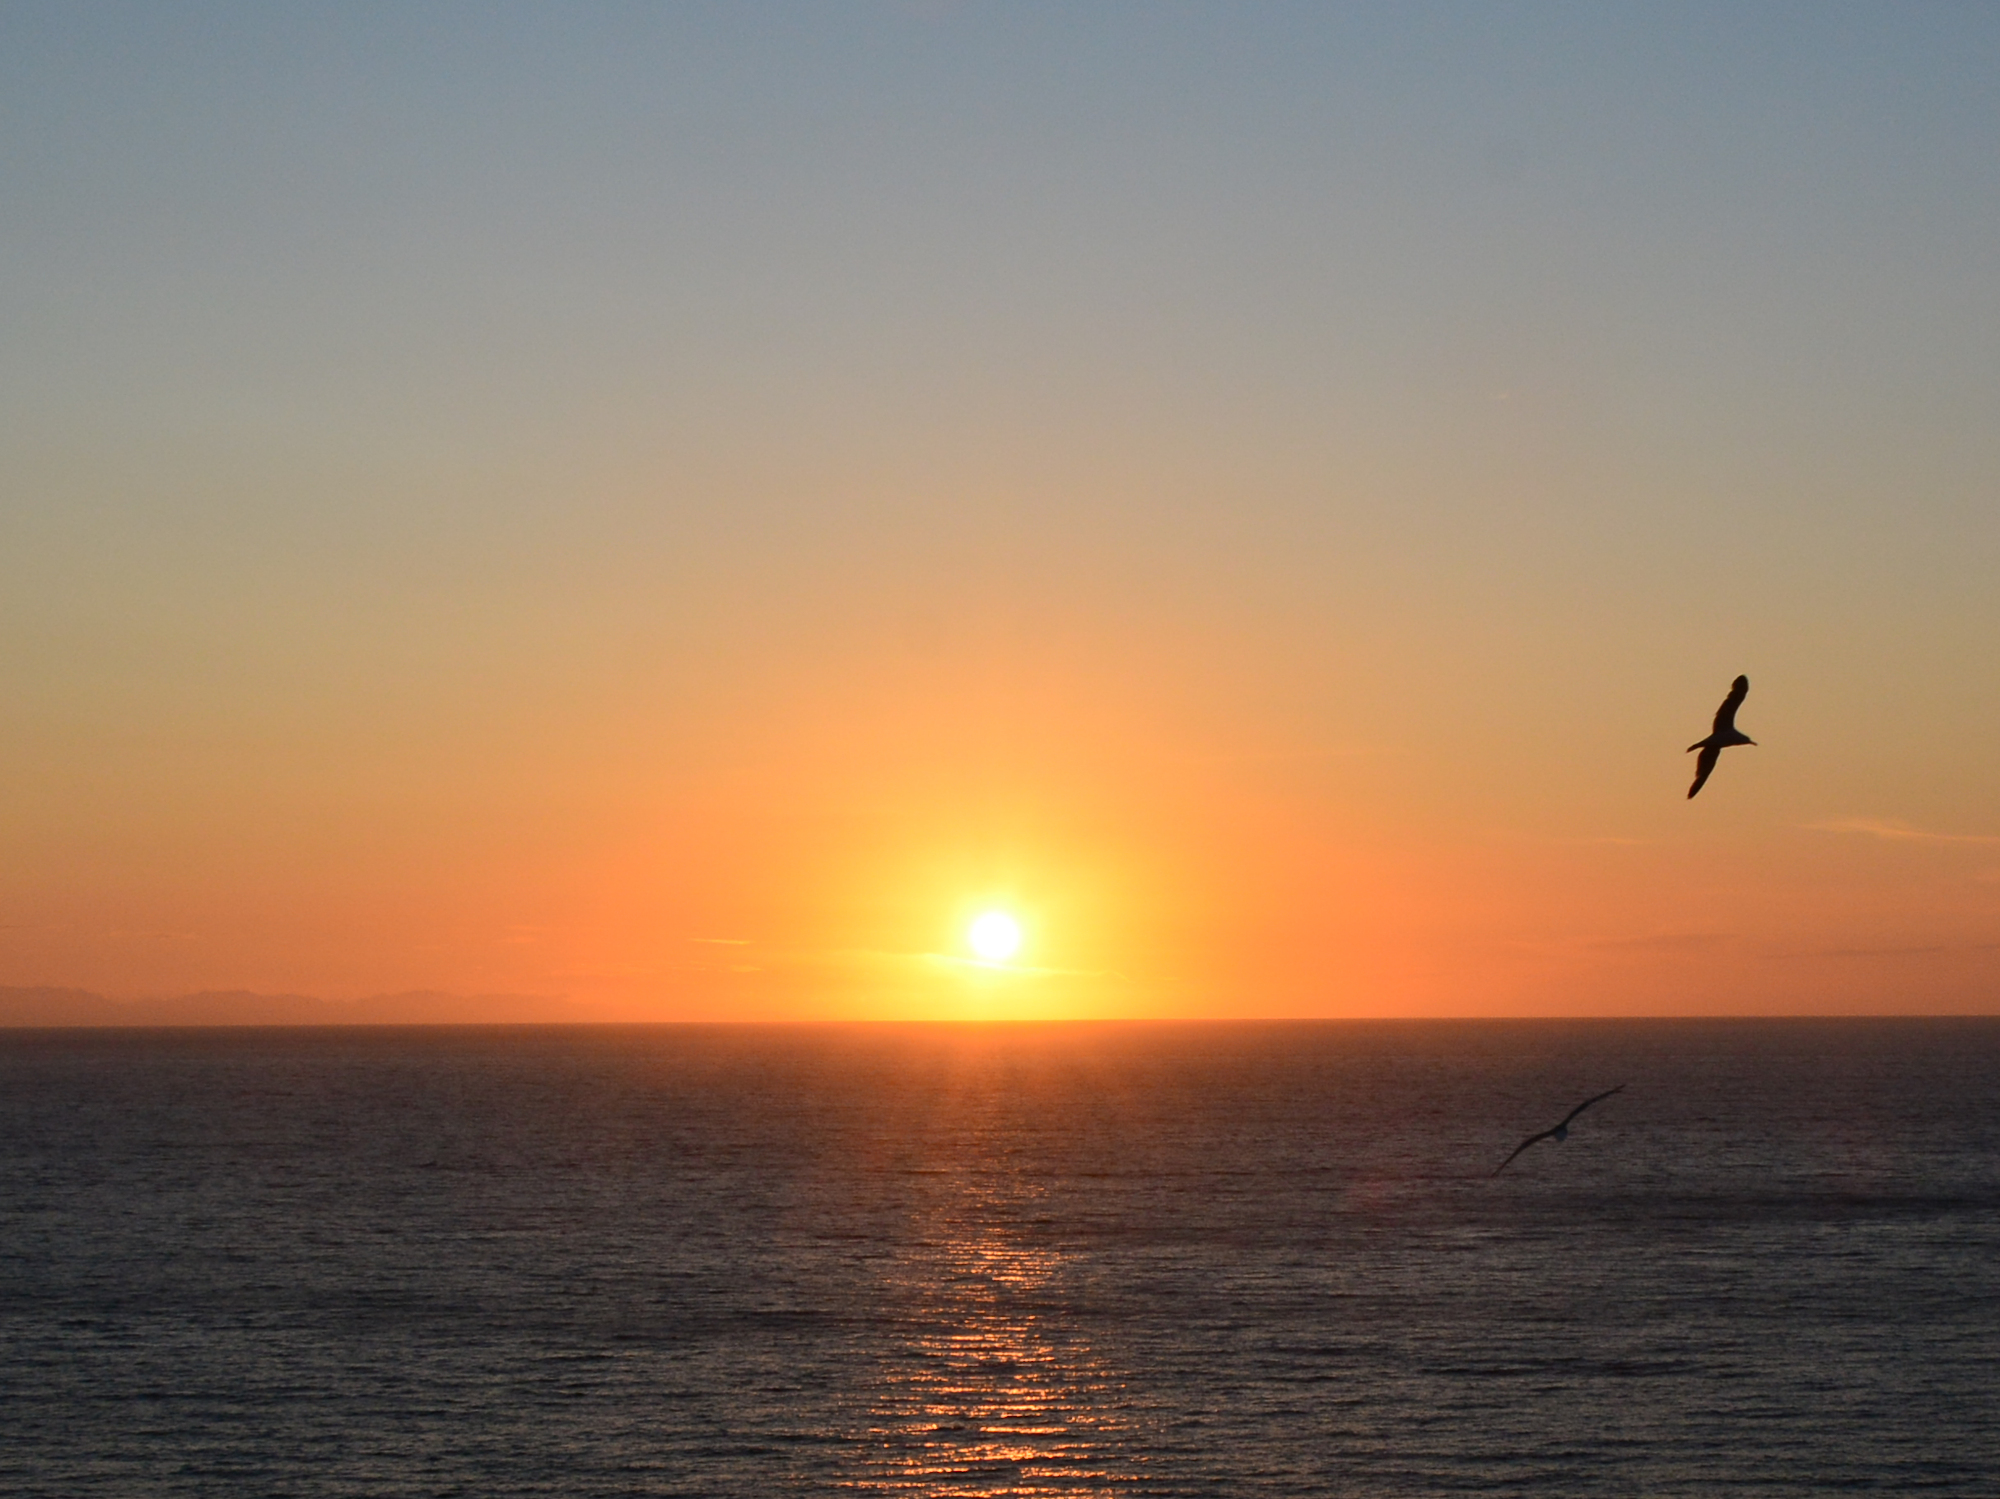
\includegraphics[width=7truecm]{slike/07_Zahod.jpg}\hfill
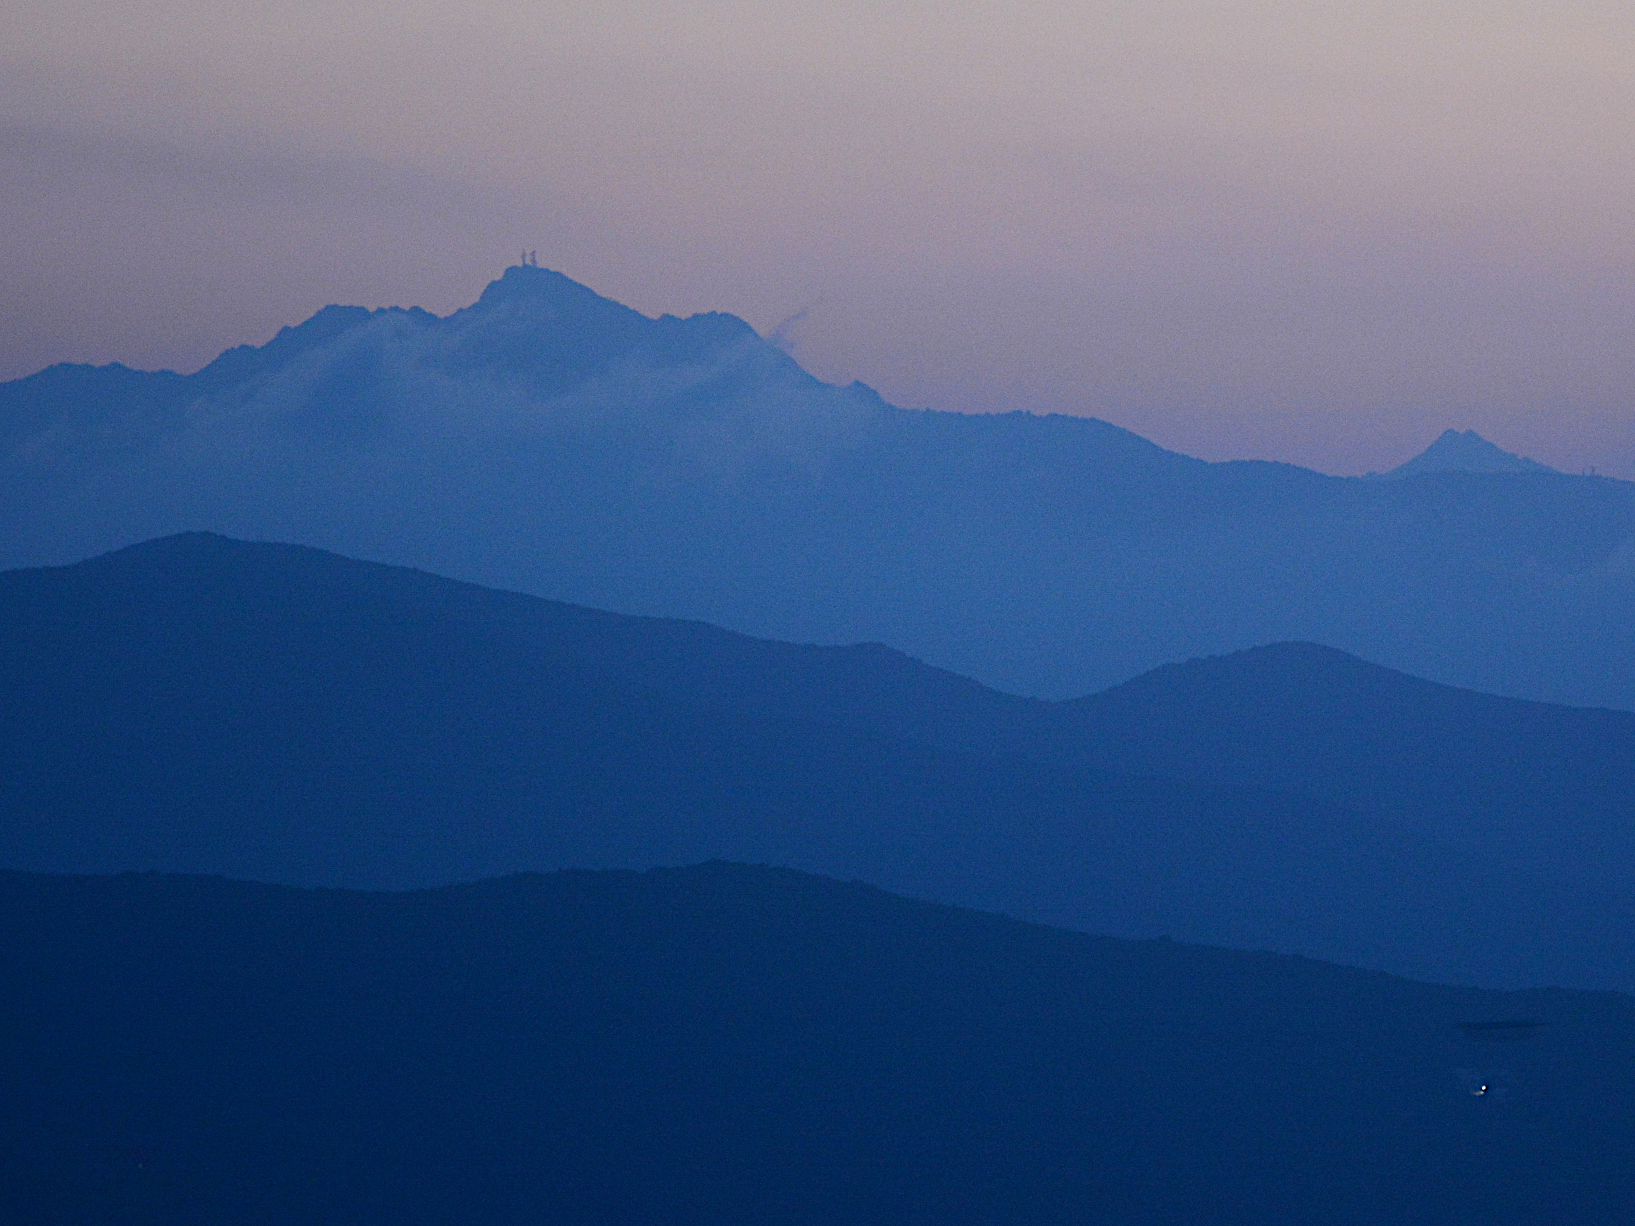
\includegraphics[width=7truecm]{slike/07_Hribi.jpg}
\caption{Ker se modra barva bolj siplje, je večina prepuščene svetlobe ob sončnem
vzhodu ali zahodu rdečkaste barve (levo). Sipanje svetlobe je vzrok, zakaj so oddaljeni
grebeni videti modrikastih barv (desno).}
\label{fig:07_Rdeca}
\end{figure}

\begin{example}{\bf Zakaj so oddaljene gore modikaste?}
Zaradi sipanja svetlobe v zraku opazimo še en zanimiv pojav: modrikasto
obarvanost oddaljenih gorskih grebenov. Med opazovalcem in oddaljenim grebenom
je razmeroma dolga pot skozi ozračje, na katerem se svetloba siplje. Več kot
je ozračja med goro in opazovalcem, več bo sipane svetlobe. Posledično so
bolj oddaljene gore videti bolj modro in svetlejše (slika~\ref{fig:07_Rdeca}, desno). 

Kadar ozračje ni čisto in so prisotni večji delci (na primer prah ali vodne kapljice),
takrat se svetloba siplje drugače. Kot bomo spoznali v nadaljevanju, je sipanje
na večjih delcih le šibko odvisno od valovne dolžine svetlobe, zato je svetloba, sipana
na večjih delcih, siva. V meglenem vremenu so posledično oddaljene gore -- in celo nebo -- 
videti sivo.
\end{example}

\begin{example}{\bf Tyndallov pojav.} Tyndallov pojav, ki se imenuje po irskem fiziku\index{Tyndall, John}
Johnu Tyndallu (1820--1893), opisuje sipanje svetlobe v koloidih in suspenzijah.\index{Tyndallov pojav}
Za Rayleighovo
sipanje smo izpeljali, da intenziteta sipane svetlobe narašča s šesto potenco velikosti
delca (enačba~\ref{eq:07_17}). Na večjih delcih (a po velikosti še vedno manjših 
ali največ primerljivih z valovno dolžino 
svetlobe), se tako svetloba zelo močno siplje. Koloide pri navadni 
osvetlitvi zato pogosto vidimo modrikaste, pri presevni osvetlitvi pa rdečkaste barve.
\begin{figure}[!ht]
\centering
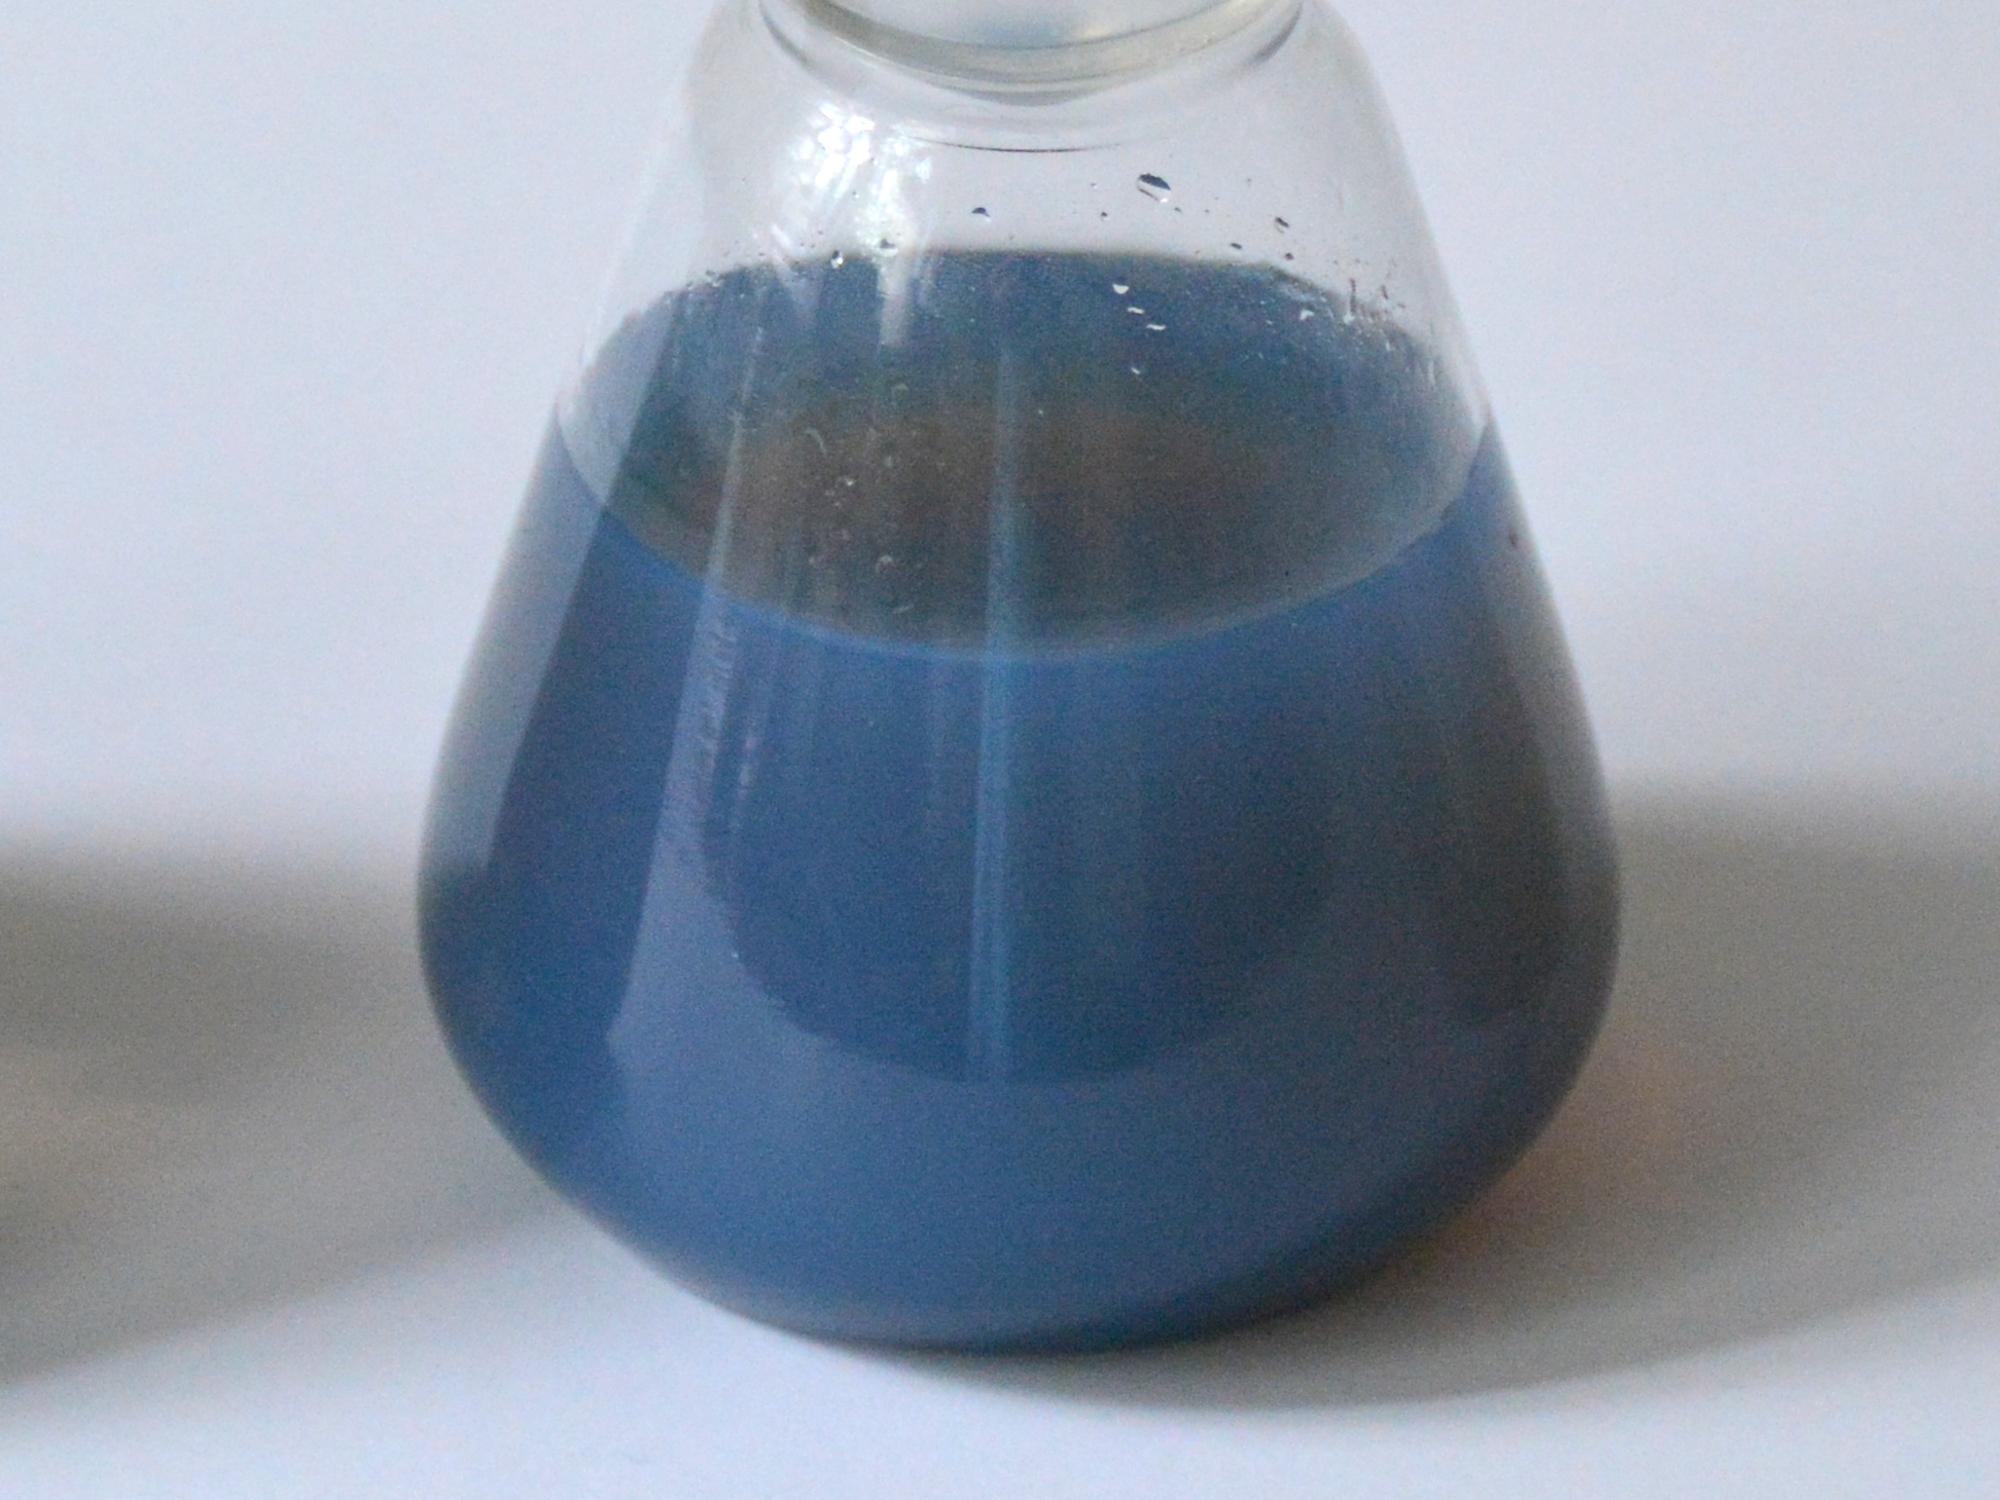
\includegraphics[width=7truecm]{slike/07_Mo2N1.jpg}\hfill
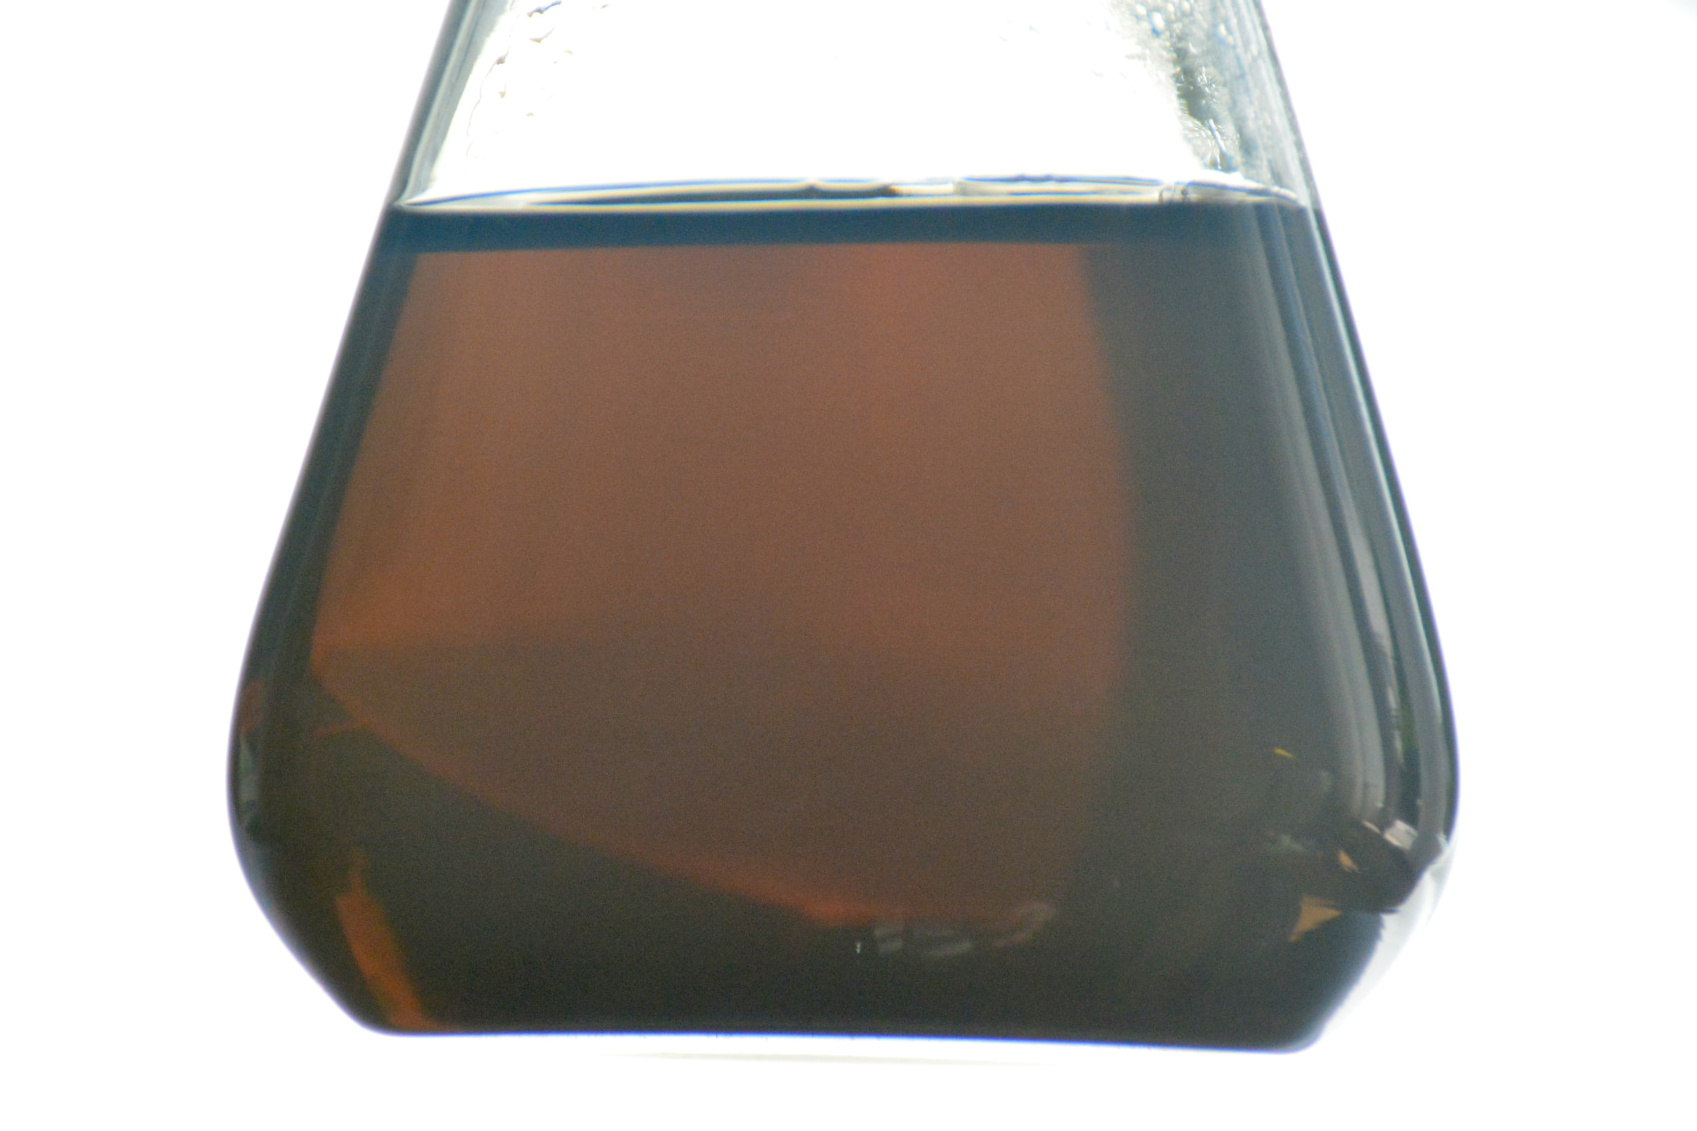
\includegraphics[width=7truecm]{slike/07_Mo2N2.jpg}
\caption{Disperzije nanodelcev molibdenovega nitrida v vodi, ki je zaradi sipanja
videti modra (levo). Ko isto disperzijo osvetlimo od zadaj, je prepuščena svetloba rdečkasta
(desno).}
\label{fig:07_Tyndall}
\vglue-10truemm
\end{figure}

\end{example}

\section{Polarizacija sipane svetlobe}\index{Polarizacija!{sipane svetlobe}}\index{Sipanje!{polarizacija}}
Pri razlagi Rayleighovega sipanja v prejšnjem razdelku smo privzeli, da na
delec vpada linearno polarizirano elektromagnetno valovanje, ki v delcu vzbudi 
električni dipolni moment. Oscilirajoči dipol seva, pri čemer je polarizacija
izsevane svetlobe vzdolž enotskega vektorja $\mathbf{e}_\vartheta$. Sevanja vzdolž
smeri vpadne polarizacije ni, v smeri pravokotno na vpadno svetlobo pa je polarizacija
pravokotna na sipalno ravnino (slika~\ref{fig:07_pol}\,a).

Kadar na sipalni delec vpada nepolarizirana svetloba, vpadno svetlobo razstavimo\index{Sipanje!{nepolarizirane svetlobe}}
na dve med seboj pravokotni komponenti in obravnavamo vsako posebej. Naj bo smer
vpadne svetlobe vzdolž osi $x$, električno polje vpadne svetlobe pa razdelimo na 
polarizacijo vzdolž osi $y$ in polarizacijo vzdolž osi $z$ (slika~\ref{fig:07_pol}\,b).  
Komponenta vzdolž osi $y$ vzbudi dipolni moment, ki vzdolž osi $y$ 
ne seva, vzdolž osi $z$ pa je izsevana svetloba polarizirana v smeri $y$. 
Podobno komponenta vzdolž osi $z$ ne povzroči sevanja vzdolž osi $z$,
izsevana svetloba vzdolž osi $y$ pa je polarizirana v smeri $z$. Posledično je v smereh
pravokotno na smer vpadne svetlobe sipana svetloba linearno polarizirana. 
Pri poljubnem sipalnem kotu je sipana svetloba na splošno delno polarizirana.
\begin{figure}[!ht]
\centering
\def\svgwidth{135truemm} 
\input{slike/07_sipanjePol_1.pdf_tex}
\caption{Linearno polarizirana vpadna svetloba se na delcu siplje, pri čemer je polarizacija
sipane svetlobe vzporedna z $\mathbf{e}_\vartheta$ (a). Nepolarizirano vpadno svetlobo
razstavimo na dve komponenti (rdeča in modra) in ju obravnavamo neodvisno. 
V smeri pravokotno na vpadno svetlobo je sipana svetloba linearno polarizirana, na splošno
pa delno polarizirana.}
\label{fig:07_pol}
\vglue-5truemm
\end{figure}

Poglejmo pojav podrobneje. Naj bo opazovalec vzdolž smeri vektorja $\mathbf{r}$, katerega
smer določajo koti $\vartheta_1$, $\vartheta_2$ in $\beta$. Pri tem je $\vartheta_1$ 
kot med smerjo opazovalca in osjo $y$, $\vartheta_2$ med smerjo opazovalca in 
osjo $z$, kot $\beta$, tako imenovani sipalni kot, pa je kot med smerjo opazovalca 
in osjo $x$ (slika~\ref{fig:07_smernikoti}). Med koti velja\index{Sipalni kot}
zveza: $\cos^2 \vartheta_1 + \cos^2 \vartheta_2 + \cos^2 \beta = 1$.
\begin{figure}[!ht]
\vglue-2truemm
\centering
\def\svgwidth{50truemm} 
\input{slike/07_smernikoti.pdf_tex}
\caption{Smer opazovalca $\mathbf{r}$ označimo s tremi koti glede na koordinatne osi.}
\label{fig:07_smernikoti}
\vglue-5truemm
\end{figure}

Sevalno polje dipola, induciranega v smeri $y$ 
zapišemo kot (enačba~\ref{eq:07_53}):
\begin{equation}
j_y = \frac{j_0}{2} f(\omega, r) \sin^2 \vartheta_1.
\label{eq:07_58}
\end{equation}
Konstante ter odvisnost od frekvence in oddaljenosti od dipola smo združili 
v funkcijo $f$. Upoštevali smo le polovico gostote vpadnega svetlobnega toka $j_0$, saj 
velja zapisano le za izbrano polarizacijo. Podobno zapišemo sevalno polje dipola, ki je 
induciran v smeri $z$:
\begin{equation}
j_z = \frac{j_0}{2} f(\omega, r) \sin^2 \vartheta_2.
\label{eq:07_59}
\end{equation}
Celotna gostota energijskega toka sipane svetlobe je vsota obeh prispevkov:
\begin{equation}
j_\mathrm{sev} = j_y + j_z = j_0 f(\omega, r) \frac{\sin^2 \vartheta_1 + \sin^2 \vartheta_2}{2}.
\label{eq:07_60}
\end{equation}
Z upoštevanjem zveze med smernimi kosinusi dobimo:
\boxeq{eq:07_61}{
j_\mathrm{sev} = j_0 f(\omega, r) \frac{1+ \cos^2 \beta}{2}.
}
Intenziteta sipane nepolarizirane svetlobe je, po pričakovanju, odvisna zgolj od sipalnega kota $\beta$.
Njena odvisnost (slika~\ref{fig:07_nepol}) je simetrična v smeri naprej in nazaj, pri čemer je 
sipanja v teh dveh smereh dvakrat več kot pravokotno na vpadno smer. V smeri naprej je sipanje 
nepolarizirano, v pravokotnih smereh je linearno polarizirano, v ostalih smereh pa delno polarizirano.
\begin{figure}[!ht]
\vglue-2truemm
\centering
\def\svgwidth{70truemm} 
\input{slike/07_nepol.pdf_tex}
\caption{Celotna intenziteta sipane nepolarizirane svetlobe je vsota dveh prispevkov, pri čemer vsak
ustreza eni od komponent polarizacije vpadne svetlobe (modra $y$ in rdeča $z$). Prostorska porazdelitev
intenzitete sipane svetlobe je osno simetrična okoli osi $x$.}
\label{fig:07_nepol}
\vglue-7truemm
\end{figure}

\begin{example}{\bf Sipanje polarizirane svetlobe.} Posvetimo z linearno polarizirano
svetlobo v posodico z vodo, kateri smo dodali kapljico mleka. Svetloba se siplje,
vendar je intenziteta sipane svetlobe na mestu opazovalca močno odvisna
od smeri vpadne polarizacije. Z zasukom laserja za $90\si{\degree}$
sipana svetloba praktično izgine (sliki~\ref{fig:07_mleko} zgoraj). 
Polarizacijo sipane svetlobe preverimo z uporabo linearnih polarizatorjev 
(sliki~\ref{fig:07_mleko} spodaj). 
\begin{figure}[!ht]
\centering
\vglue-1truemm
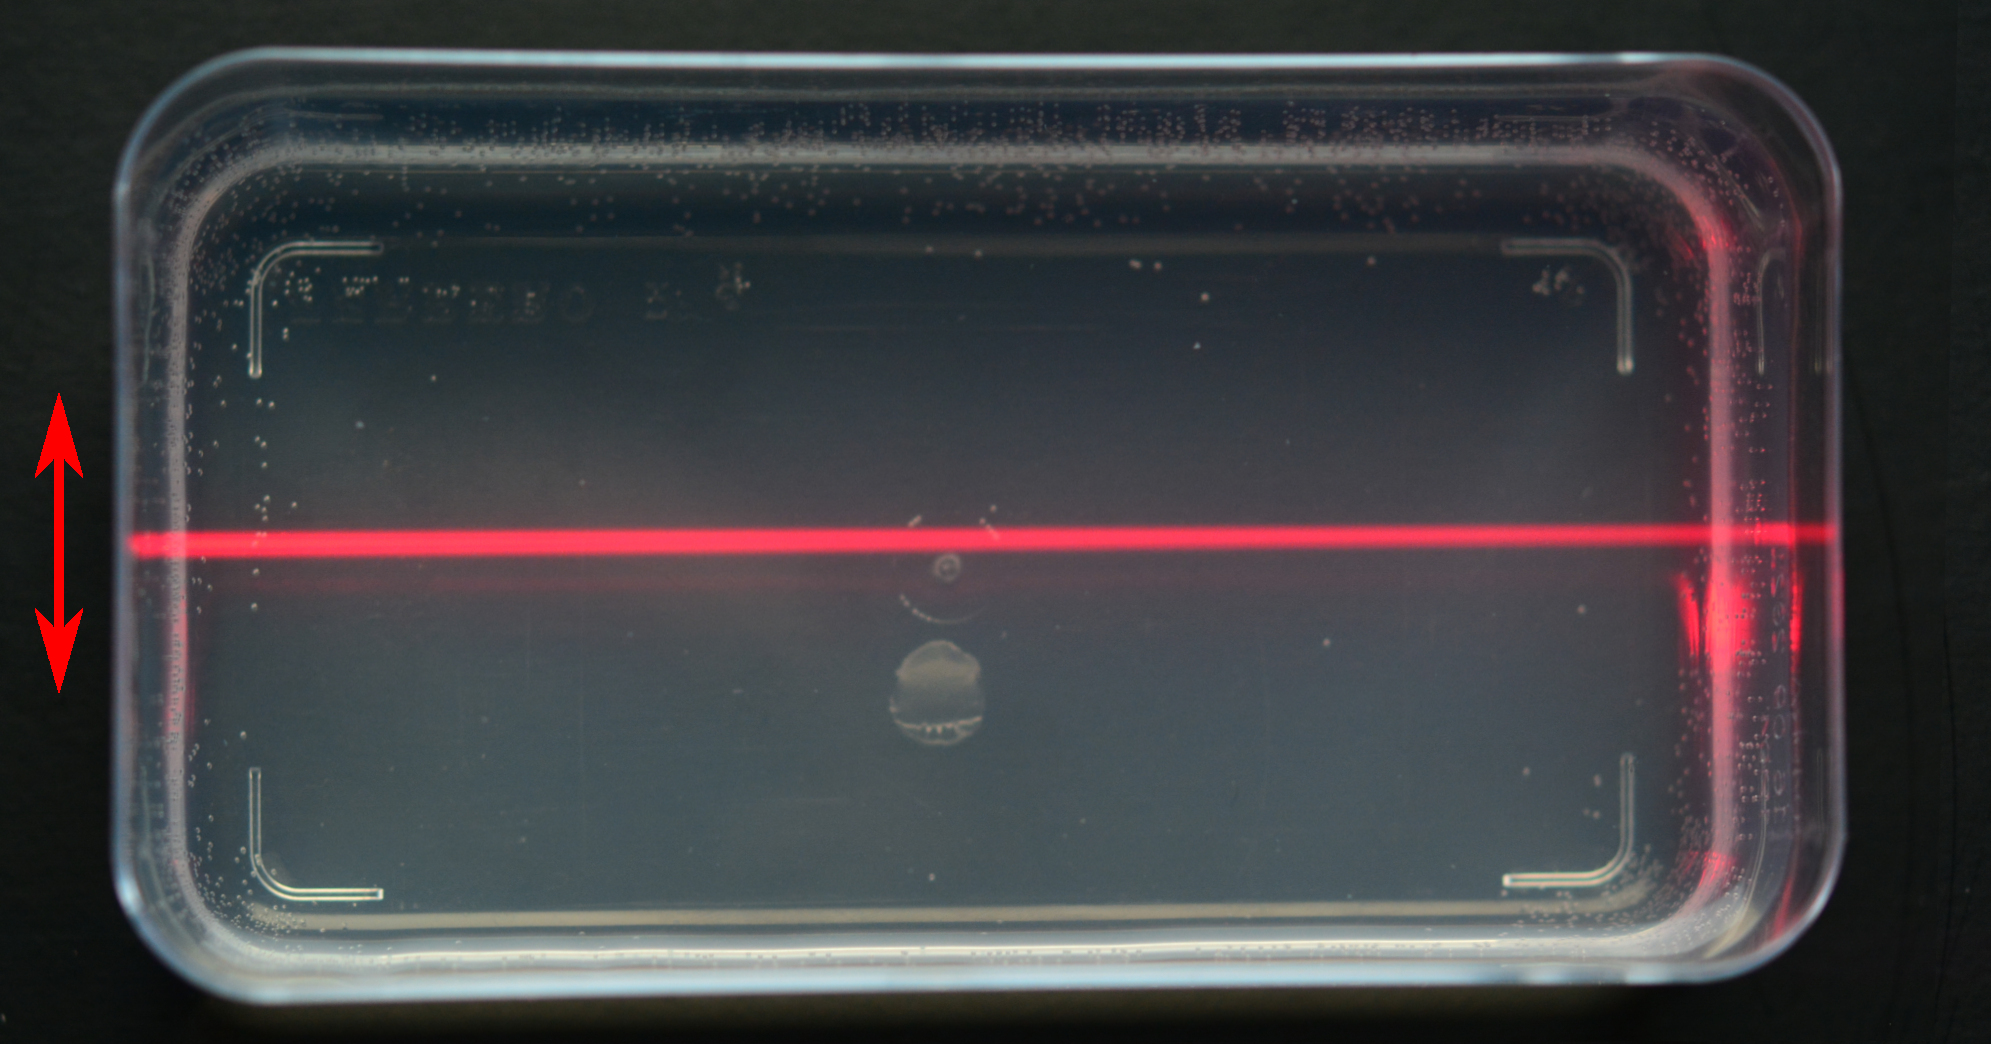
\includegraphics[width=7truecm]{slike/07_Mleko1.jpg}\hfill
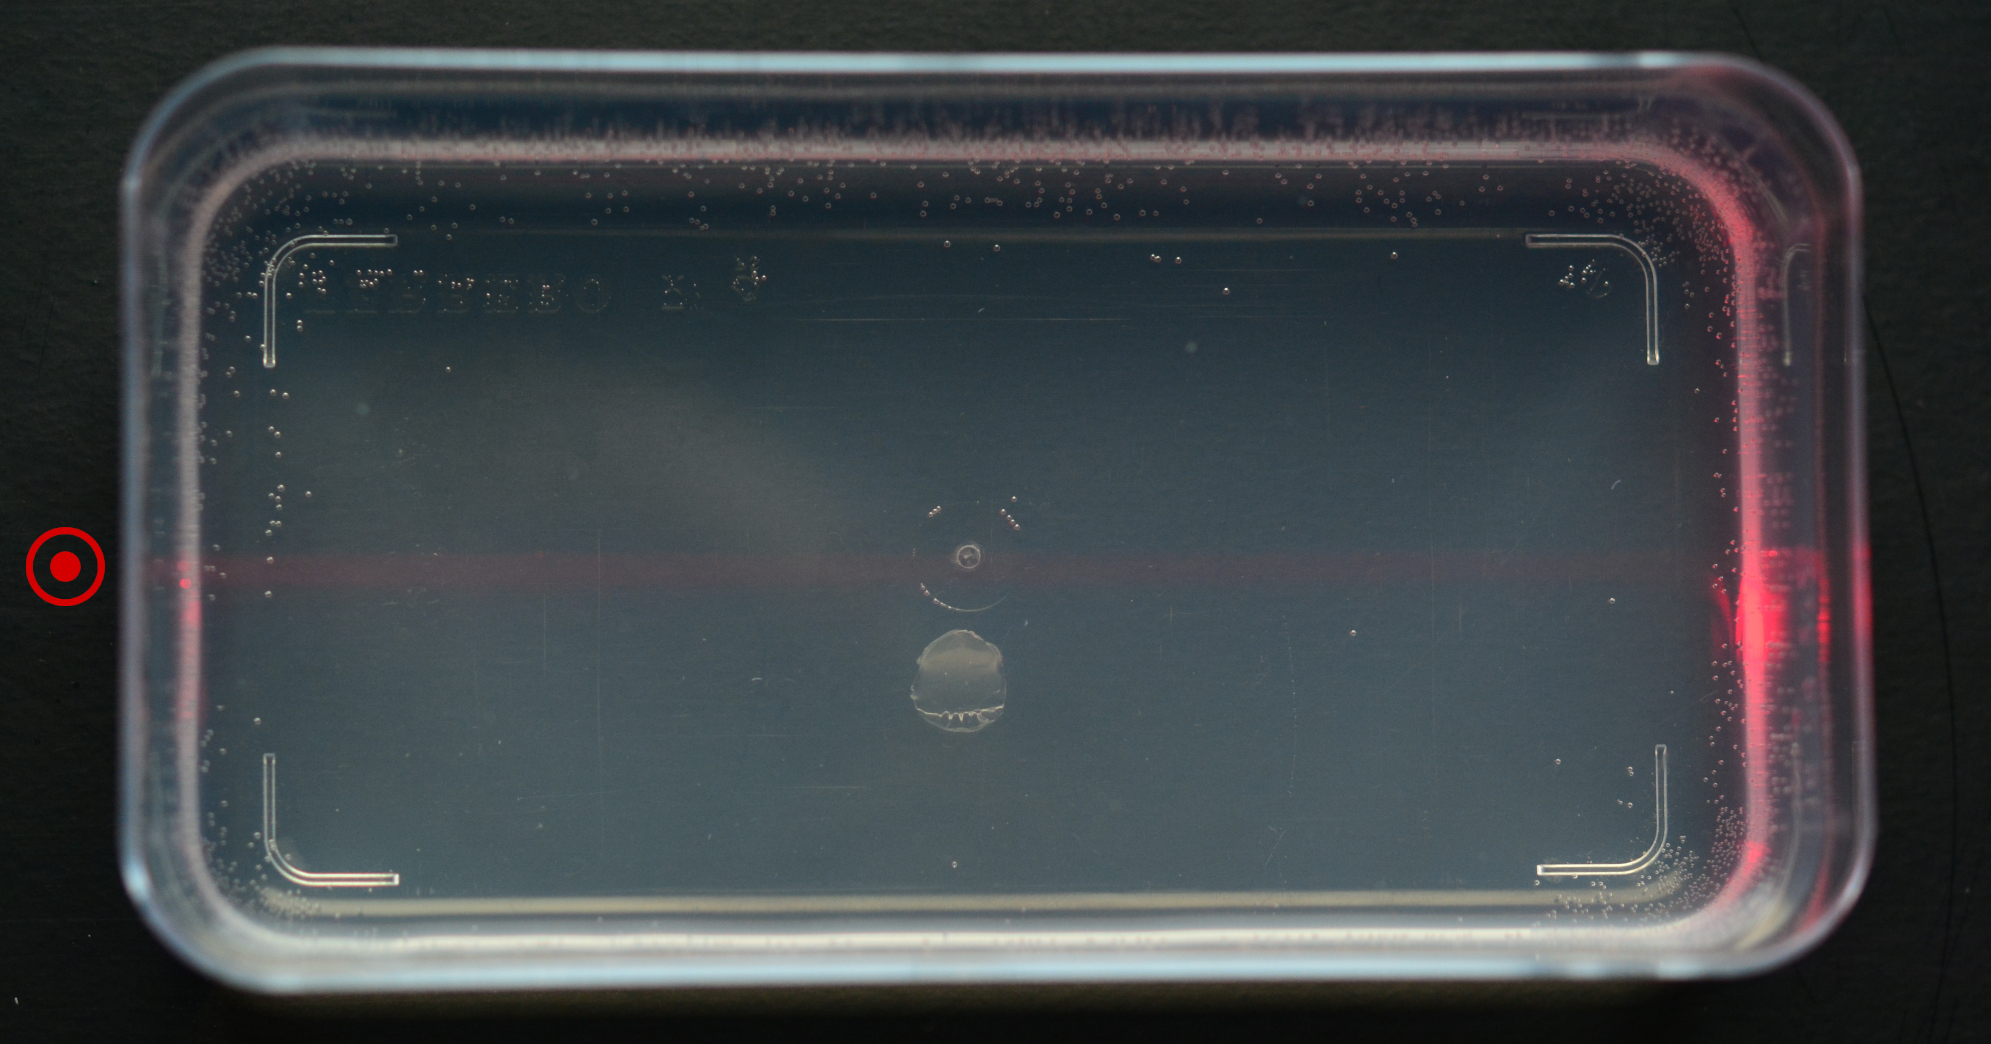
\includegraphics[width=7truecm]{slike/07_Mleko2.jpg}\\ \vglue3truemm
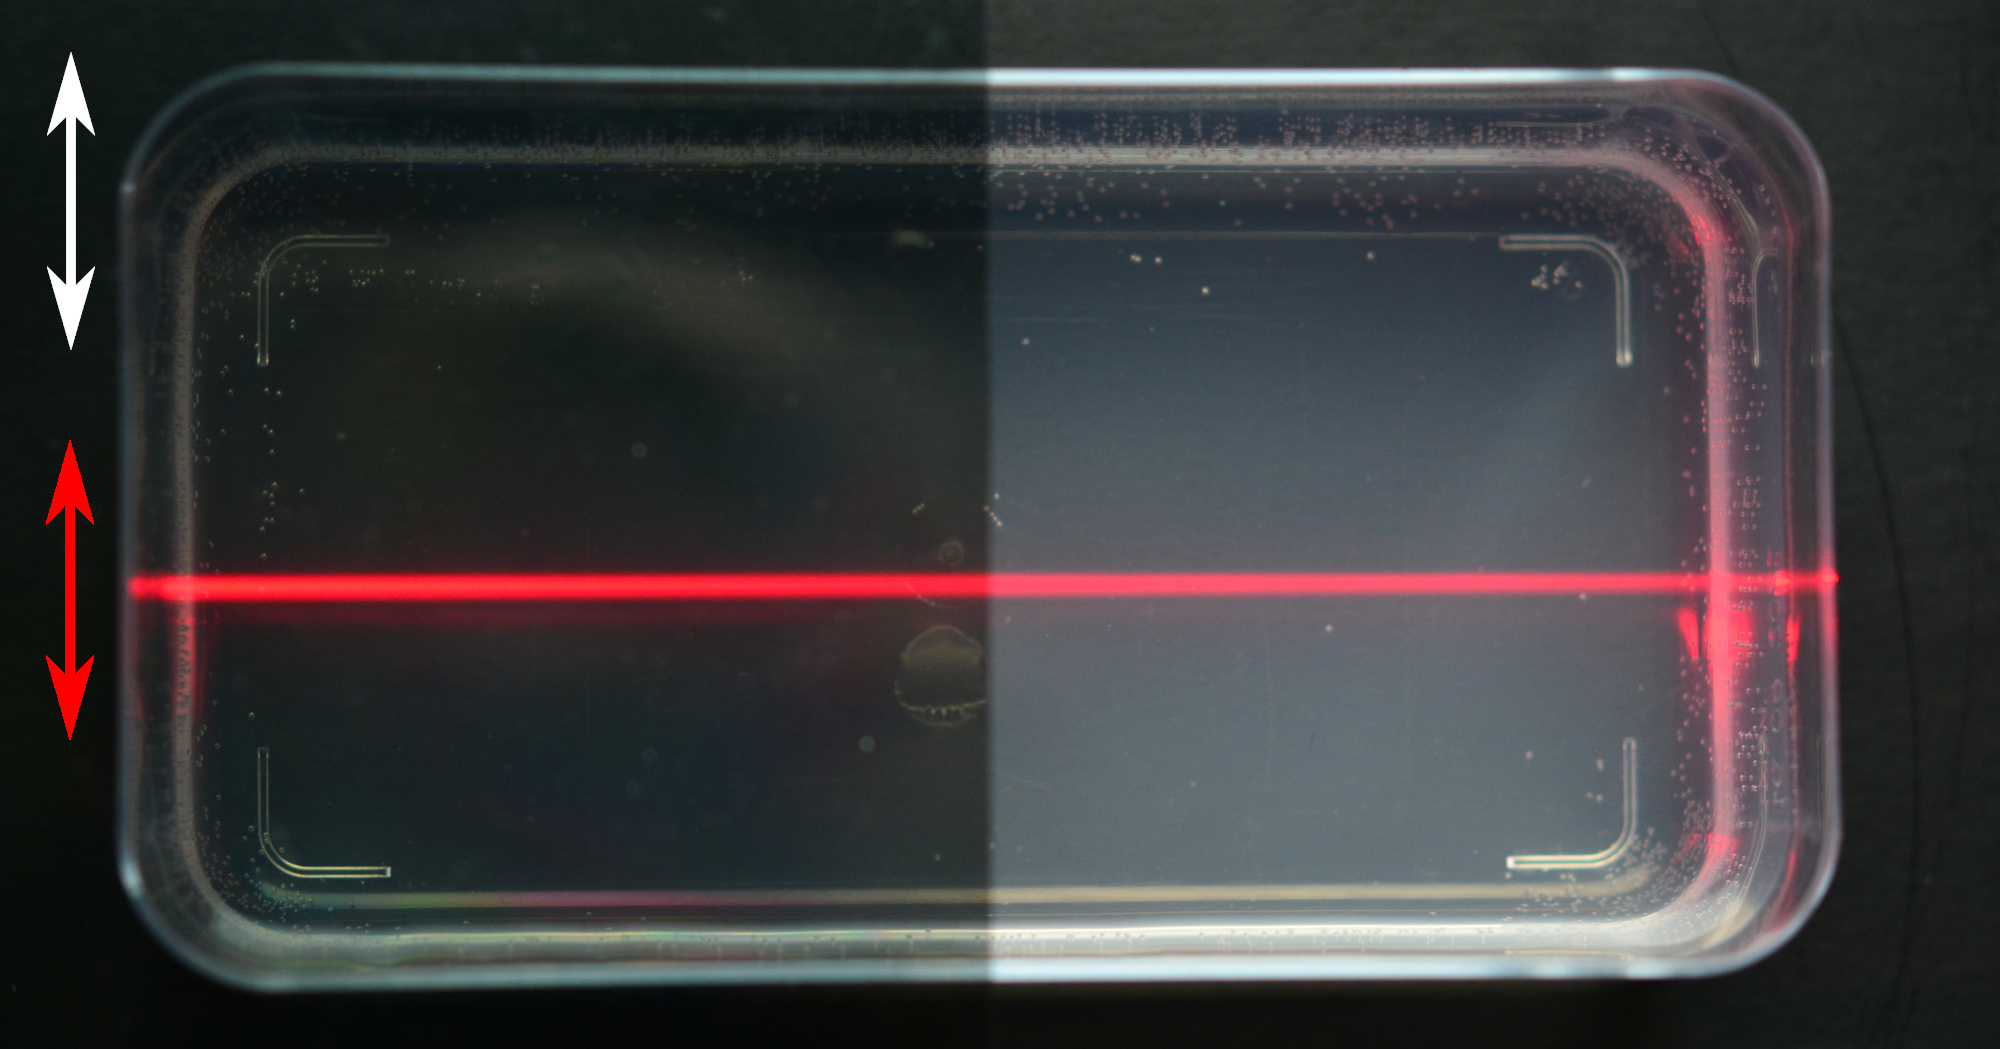
\includegraphics[width=7truecm]{slike/07_Mleko3.jpg}\hfill
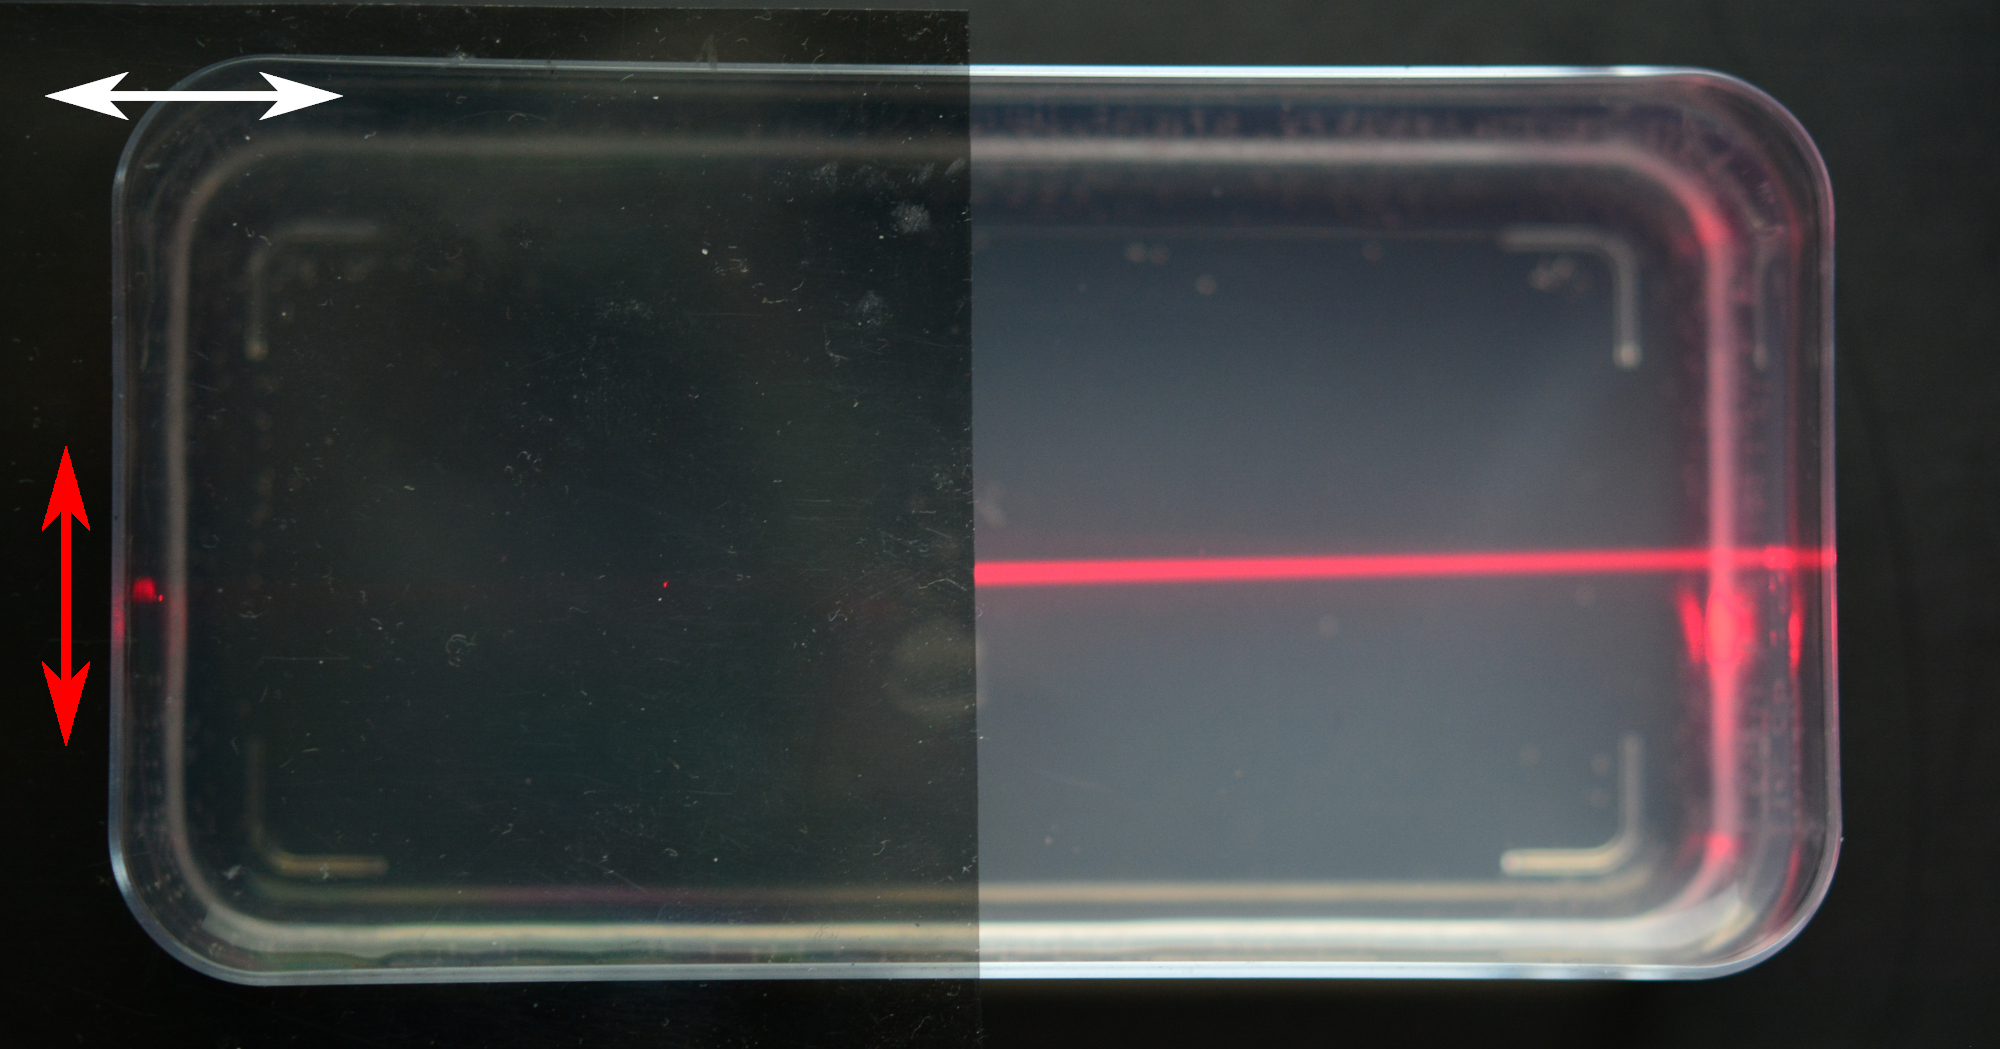
\includegraphics[width=7truecm]{slike/07_Mleko4.jpg}
\caption{Sipanje v posodici vode z dodano kapljivo mleka. Intenziteta sipane svetlobe je odvisna 
od polarizacije vpadne svetlobe (zgoraj), sipana svetloba pod pravim kotom pa je linearno
polarizirana (spodaj). Rdeče puščice označujejo smer polarizacije svetlobe, beli puščici
pa smeri polarizatorjev.}
\label{fig:07_mleko}
\vglue-10truemm
\end{figure}

\end{example}

\begin{example}{\bf Polarizacija modrega neba.}\index{Modro nebo}
Spoznali smo, da je sipana svetloba najbolj izrazito linearno polarizirana v smeri pravokotno na smer 
širjenja. Pri opazovanju neba to pomeni pravokotno na smer, iz katere vpada nepolarizirana\index{Sonce}
svetloba s Sonca. Komponenta svetlobe, ki je polarizirana pravokotno na Zemljino površje, 
v smeri opazovalca ne seva, polarizacija, ki leži tangentno na Zemljino površje, pa. Ta
pojav preverimo s polarizacijskim filtrom. Svetloba, ki jo zaznamo, tudi pri pravokotni smeri
ni povsem linearno polarizirana, saj v atmosferi prihaja do večkratnega sipanja in tudi do 
sipanja na večjih delcih v atmosferi, za katere Rayleighov približek ne velja.
\begin{figure}[!ht]
\centering
\includegraphics[width=7truecm]{slike/07_NeboPol2.jpg}\hfill
\includegraphics[width=7truecm]{slike/07_NeboPol1.jpg}
\caption{Sliki neba skozi različno zasukana linearna polarizatorja nakazujeta na delno
linearno polarizacijo sipane svetlobe. Svetloba s Sonca vpada z desne, puščici pa nakazujeta
zasuk polarizatorja.}
\label{fig:07_NeboPol}
\vglue-10truemm
\end{figure}

\end{example}

% 
% \subsection*{Sipalna matrika}
% Sipanje lahko opišemo tudi z matričnim pristopom. Splošno vpadno polarizacijo 
% razstavimo na dve komponenti: eno, ki je vzporedna s sipalno ravnino $E_\parallel$, in drugo, ki 
% je nanjo pravokotna $E_\perp$. V našem zapisu je tako $E_\parallel \parallel y$ in
% $E_\perp \parallel z$. 
% \begin{equation}
% \mathbf{E}_s = 
% \left[\begin{array}{c}
% E_{s,y}\\
% E_{s,z}\\
% \end{array}\right]
% = \left[\begin{array}{c}
% E_{s, \parallel}(\beta)\\
% E_{s, \perp}(\beta)\\
% \end{array}\right] = 
% \left[\begin{array}{cc}
% S_2 & S_3 \\
% S_4 & S_1\\
% \end{array}\right] 
% \left[\begin{array}{c}
% E_{i, \parallel}\\
% E_{i, \perp}\\
% \end{array}\right] 
% \left(
% \frac{e^{ik(r-x)}}{ikr}
% \right)\!\!.
% \label{eq:07_14}
% \end{equation}
% Pri tem je matrika amplitudna sipalna matrika, ki je na splošno funkcija zenitalnega
% in azimutalnega kota (če delec ni povsem okrogel), ki poruši simetrijo. Vektor v zgornjem
% zapisu predstavlja optično polje vpadne svetlobe, zadnji člen pa je transportni faktor,
% ki je odvisen od razdalje med sipalcem in detektorjem $r$, ter od globine, v kateri
% je prišlo so sipanja (z).
% 
% V praksi navadno merimo gostoto energijskega toka sipane svetlobe:
% \begin{equation}
% j_s \propto |E_{s, \parallel}|^2 + |E_{s, \perp}|^2.
% \label{eq:07_15}
% \end{equation}
% Ker sta polarizaciji ortogonalni, mešani členi ničesar ne prispevajo. Potem sipalno matriko
% za gostoto svetlobnega toka zapišemo kot:
% \begin{equation}
% \left[\begin{array}{c}
% j_{s, \parallel}(\beta)\\
% j_{s, \perp}(\beta)\\
% \end{array}\right] = 
% \left[\begin{array}{cc}
% |S_2|^2& 0\\
% 0 & |S_1|^2\\
% \end{array}\right] 
% \left[\begin{array}{c}
% j_{i, \parallel}(\beta)\\
% j_{i, \perp}(\beta)\\
% \end{array}\right]\!\!.
% \label{eq:07_16}
% \end{equation}
% 
% .. Kakšen komentar, zakaj je to dobro, primer? .. Zakaj so indeksi tako čudno?

\section{Miejevo sipanje}\index{Miejevo sipanje}\index{Sipanje!{Miejevo}}
Z Rayleighovim sipanjem dobro opišemo sipanje svetlobe na delcih, ki so 
po velikosti precej manjši od valovne dolžine vpadne svetlobe. Po drugi strani lahko
sipanje na delcih, ki so precej večji od valovne dolžine svetlobe, opišemo
z geometrijsko optiko. V vmesnem režimu, pri katerem je velikost delcev 
primerljiva z valovno dolžino svetlobe, je opis sipanja najzahtevnejši.
Takrat govorimo o Miejevem sipanju, ki se imenuje po nemškem fiziku Gustavu 
Mieju (1868--1957). Miejevo sipanje je,\index{Mie, Gustav} 
tako kot Rayleighovo, elastično sipanje, kar pomeni, da se valovna dolžina svetlobe
pri sipanju ne spremeni.

Pri Rayleighovem sipanju smo izračunali intenziteto sipane svetlobe za posamezni
delec in prispevke vseh sipalcev sešteli. To smo lahko naredili, saj so 
zaradi naključne porazdelitve sipalcev njihovi prispevki 
statistično neodvisni in se zato seštevajo 
nekoherentno. Pri Miejevem sipanju moramo upoštevati tudi porazdelitev atomskih
sipalcev znotraj večjih delcev. Zaradi njihove vsaj delne ureditve sipljejo
svetlobo delno koherentno in do izraza pridejo interferenčni pojavi. Posledično
je kotna odvisnost Miejevo sipane svetlobe zelo zapletena. 

Druga pomembna lastnost Miejevega sipanja je zelo šibka odvisnost intenzitete
sipanja od valovne dolžine svetlobe -- za razliko od četrte potence pri Rayleighovem
sipanju. Z naraščajočo velikostjo delcev postane Miejevo sipanje neodvisno od valovne dolžine
in sipana svetloba je videti bela. Značilen primer Miejevega 
sipanja je sipanje svetlobe na drobnih kapljicah megle ali oblakov, kar da 
megli in oblakom značilno belo oziroma sivo barvo (slika~\ref{fig:07_Mie}).
\begin{figure}[!ht]
\centering
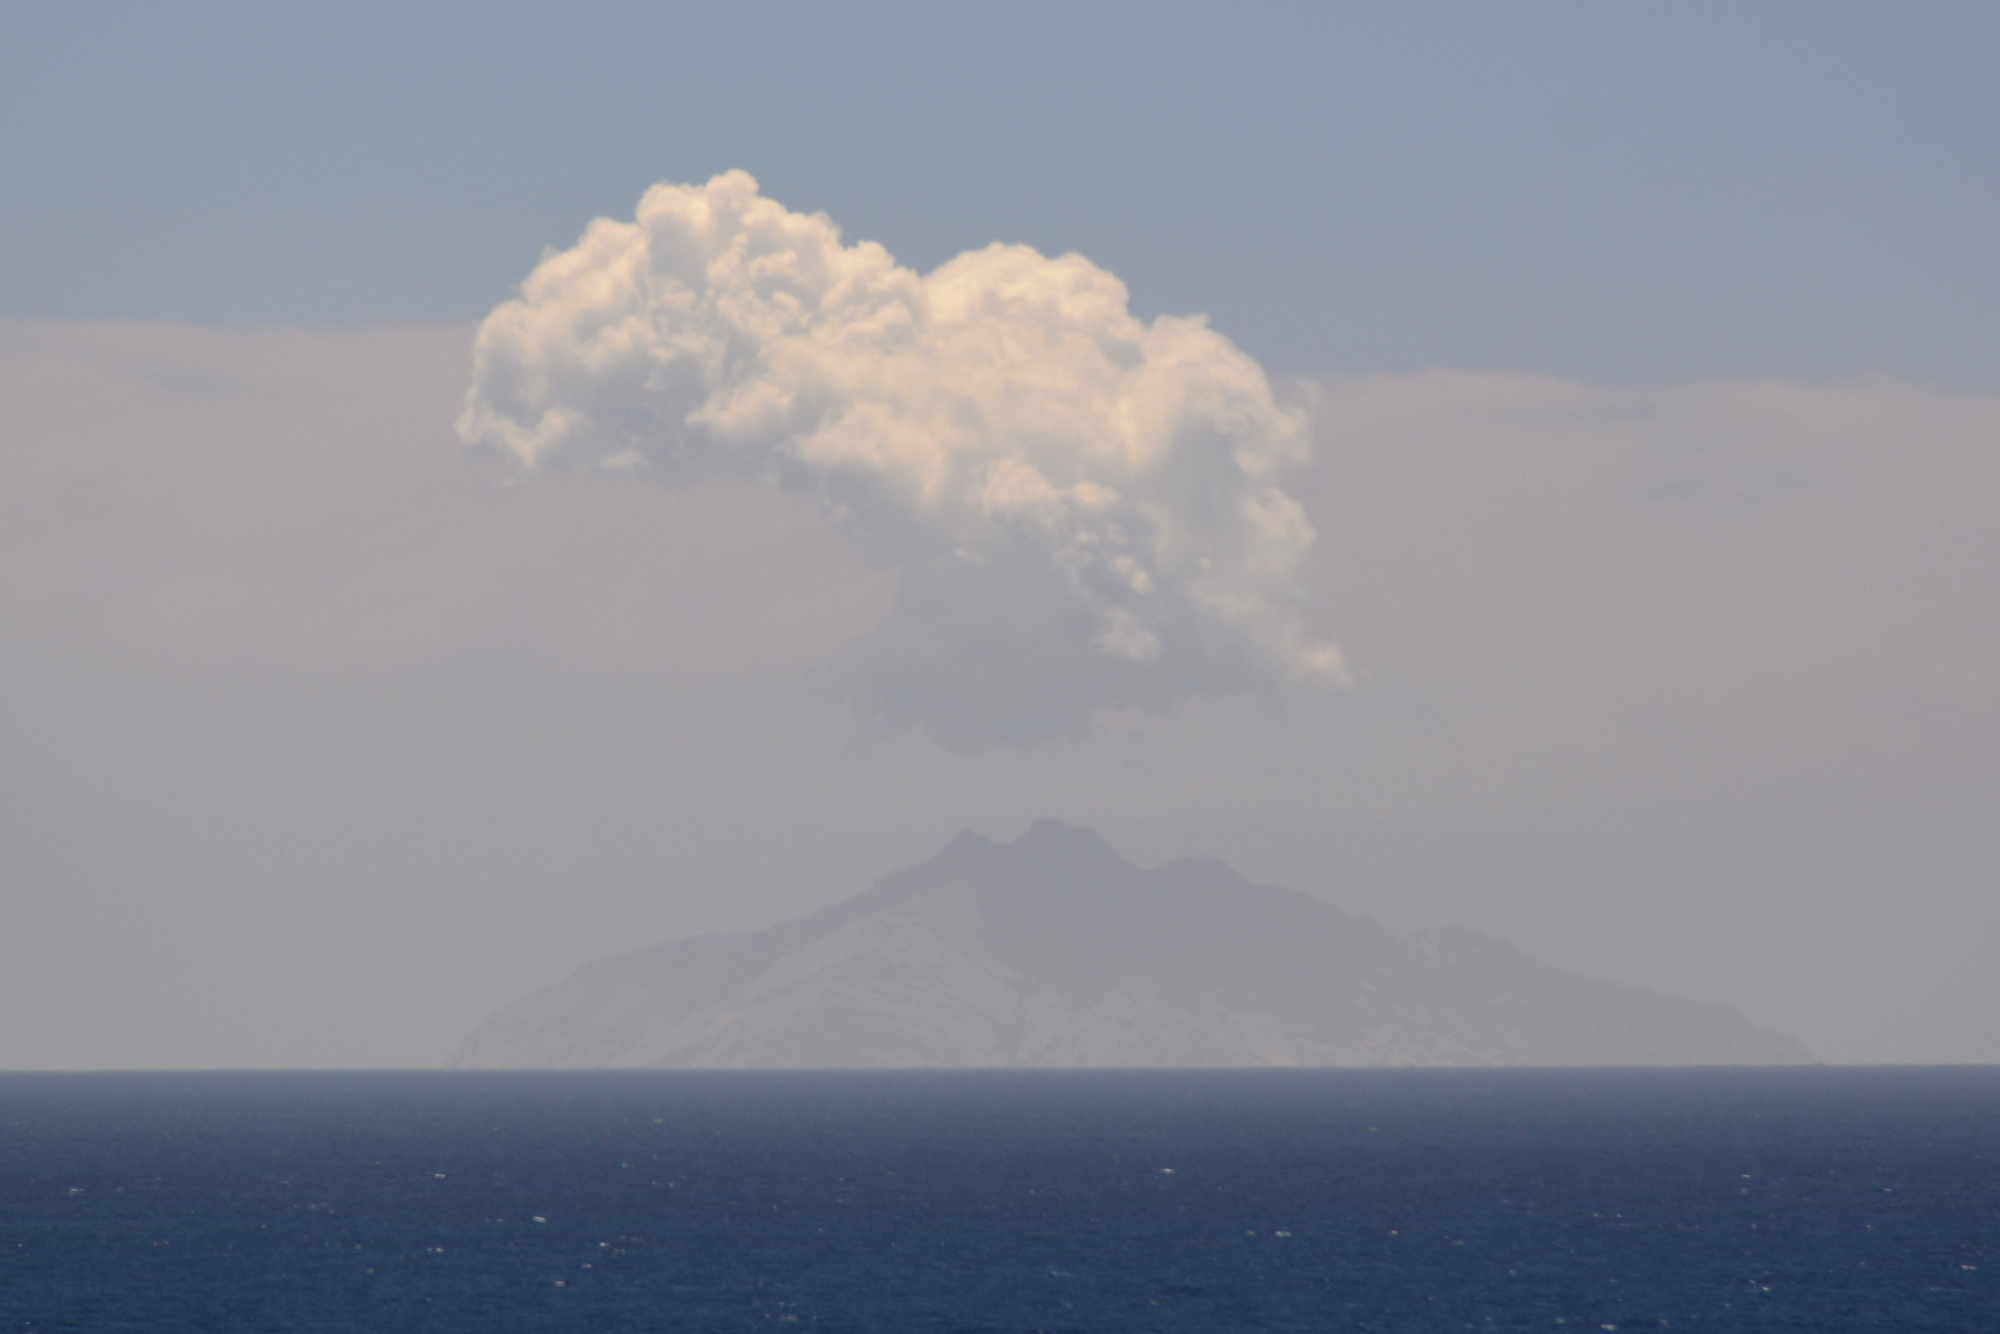
\includegraphics[width=7truecm]{slike/07_oblak.jpg}\hfill
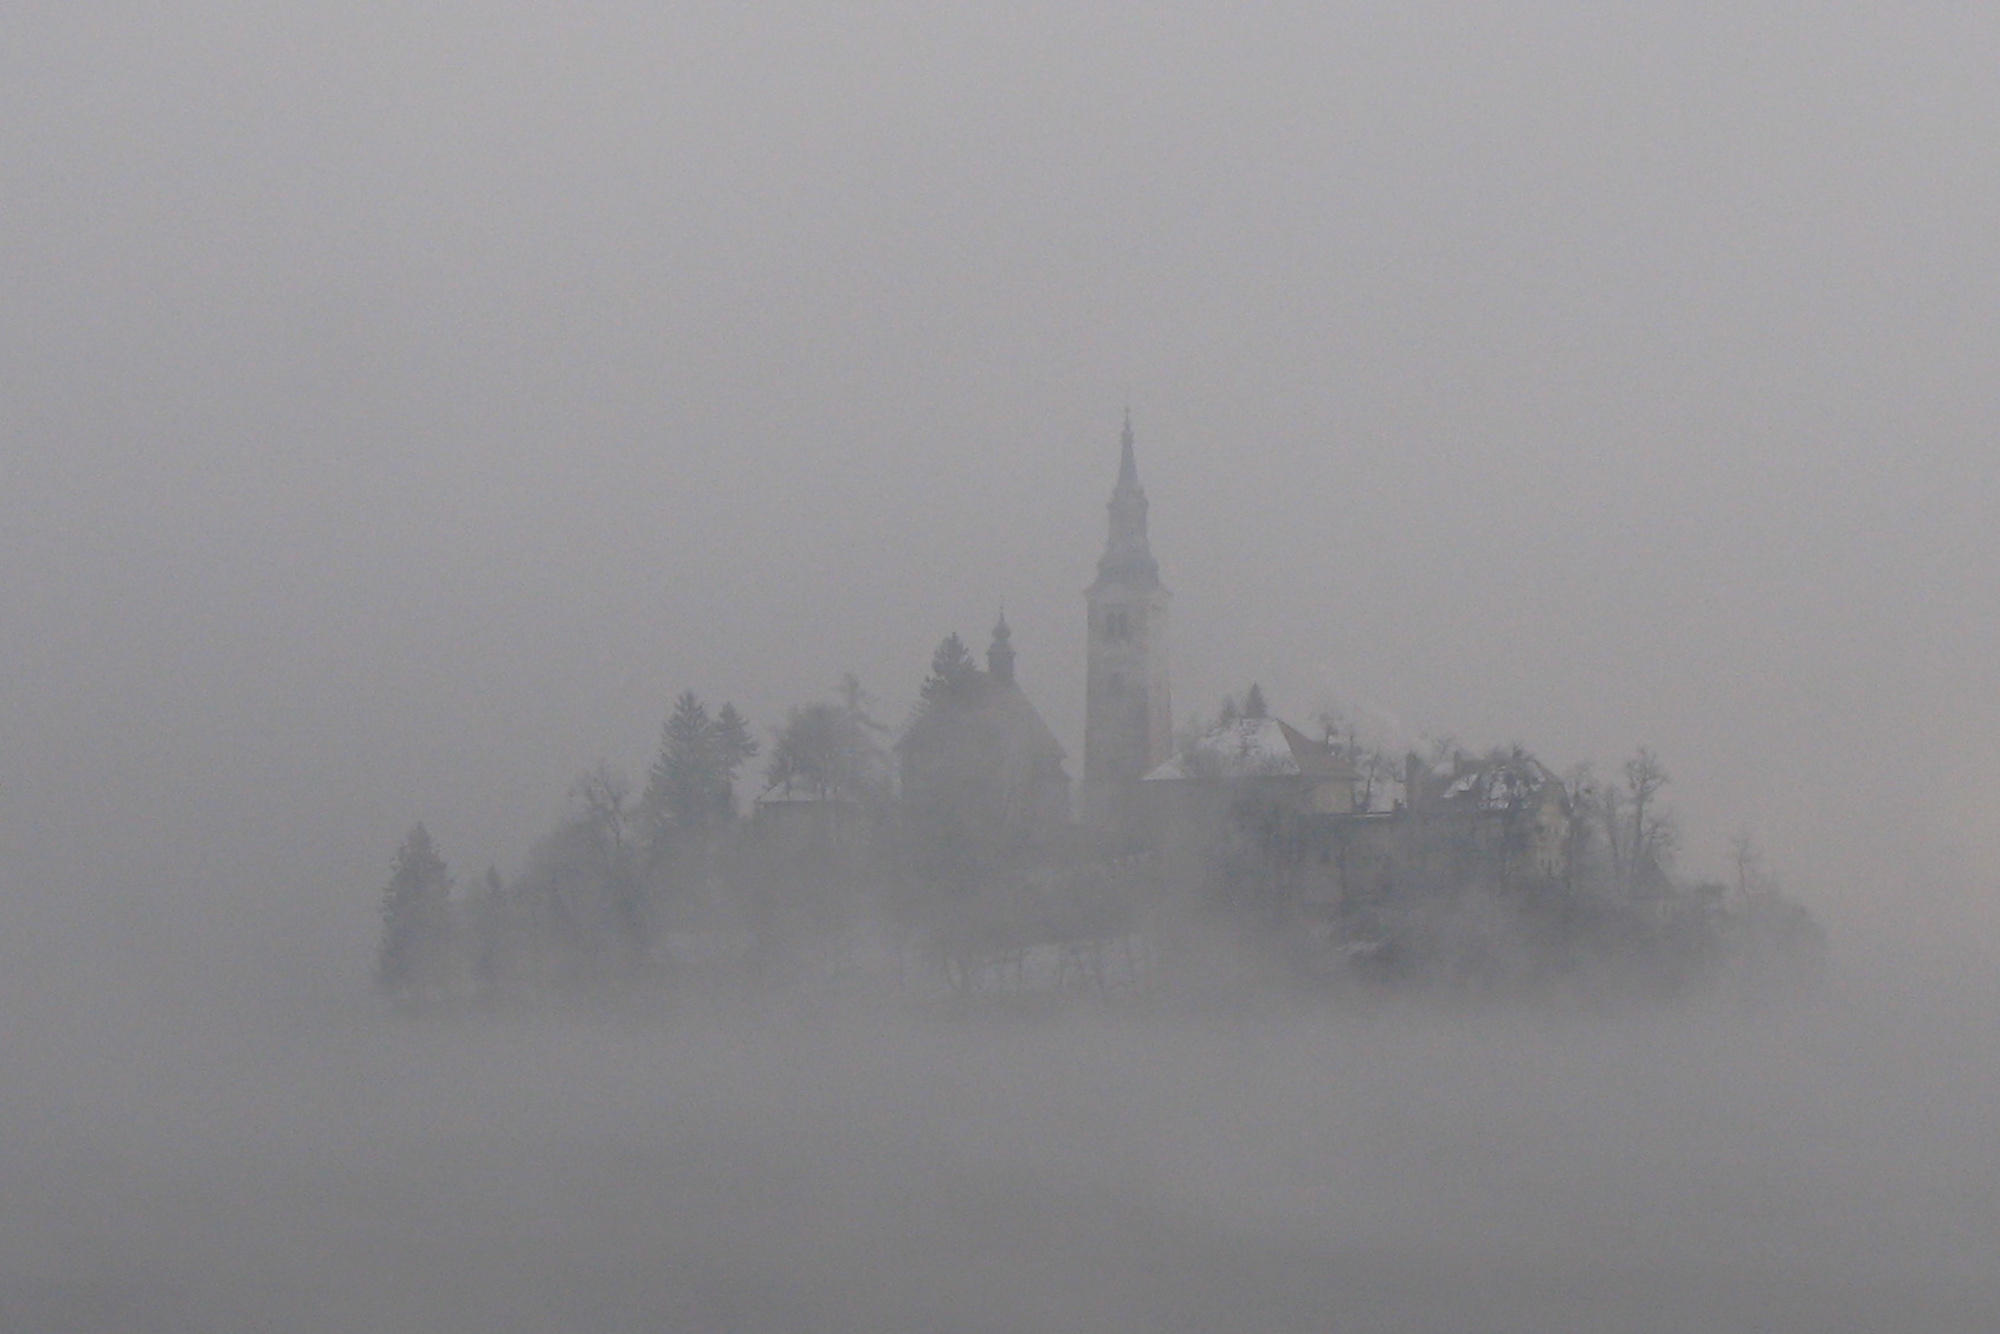
\includegraphics[width=7truecm]{slike/07_meglaB.jpg}
\caption{Oblaki (levo) in megla (desno) so videti belo zaradi sipanja svetlobe
na drobnih kapljicah vode. Pojav opišemo z Miejevim sipanjem.}
\label{fig:07_Mie}
\vglue-2truemm
\end{figure}

Izračun Miejevega sipanja na splošno poteka tako, da z reševanjem Maxwellovih enačb 
izračunamo polje znotraj in zunaj delca ter ustrezno upoštevamo robne pogoje med 
delcem in okolico. Pri tem upoštevamo velikost in obliko delca ter njegove optične
lastnosti, kot sta lomni količnik in koeficient absorpcije. Za okrogle delce 
iščemo rešitve v sferičnih koordinatah. Pojav dovolj dobro opišemo, če rešujemo skalarno
obliko Helmholtzeve enačbe (enačba~\ref{eq:03_12}) in rešitve
poiščemo z metodo separacije spremenljivk:
\begin{equation}
E_{lm}(r,\vartheta, \varphi) = 
E_0 e^{im\varphi}P_l^m (\cos \vartheta) Z_l (kr).
\label{eq:07_20}
\end{equation}
Pri tem $P$ označujejo pridružene Legendrove polinome in $Z$ sferične Besslove 
funkcije prvega ali drugega reda. Celotno sipano polje zapišemo kot vsoto vseh prispevkov:
\begin{equation}
E = \sum_{l,m} A_{lm}E_{lm},
\label{eq:07_21}
\end{equation}
pri čemer koeficiente razvoja $A_{lm}$ določimo iz robnih pogojev. 

Vpeljimo sipalni izkoristek $Q_s$ kot razmerje\index{Sipalni izkoristek}
med sipalnim presekom $\sigma_s$ in dejanskim prečnim presekom delca $A$.
Za Rayleighovo sipanje z upoštevanjem enačbe~(\ref{eq:07_17}) in prečnega preseka kroglice $\pi R^2$
izračunamo, da je sipalni izkoristek sorazmeren s četrto
potenco $kR$. Za Miejevo sipanje je ta odvisnost zaradi interferenčnih pojavov bistveno
bolj zapletena in shematsko prikazana na sliki~\ref{fig:07_MieGraf}\,a. V limiti za majhne delce
preide v Rayleighovo sipanje, v limiti velikih vrednosti $kR$ pa za delce brez 
absorpcije zavzame vrednost 2. V vmesnem območju se pojavijo vrhovi, tako imenovane Miejeve resonance, 
pri katerih je sipanje še posebej močno. Kotna odvisnost Miejevega sipanja 
(slika~\ref{fig:07_MieGraf},\,b) ima izrazit vrh v smeri naprej in zapleten vzorec 
sipanja v drugih smereh. 
\begin{figure}[!ht]
\centering
\def\svgwidth{140truemm} 
\input{slike/07_MieGraf.pdf_tex}
\caption{Sipalni izkoristek $Q_s$ za Miejevo sipanje na kroglici (a) in skica kotne porazdelitve
Miejevega sipanja (b). Povzeto po Born in Wolf, {\it Principles of Optics}, sedma izdaja, Cambridge University Press (1999).
}
\label{fig:07_MieGraf}
\vglue-3truemm
\end{figure}

\begin{figure}[!ht]
\centering
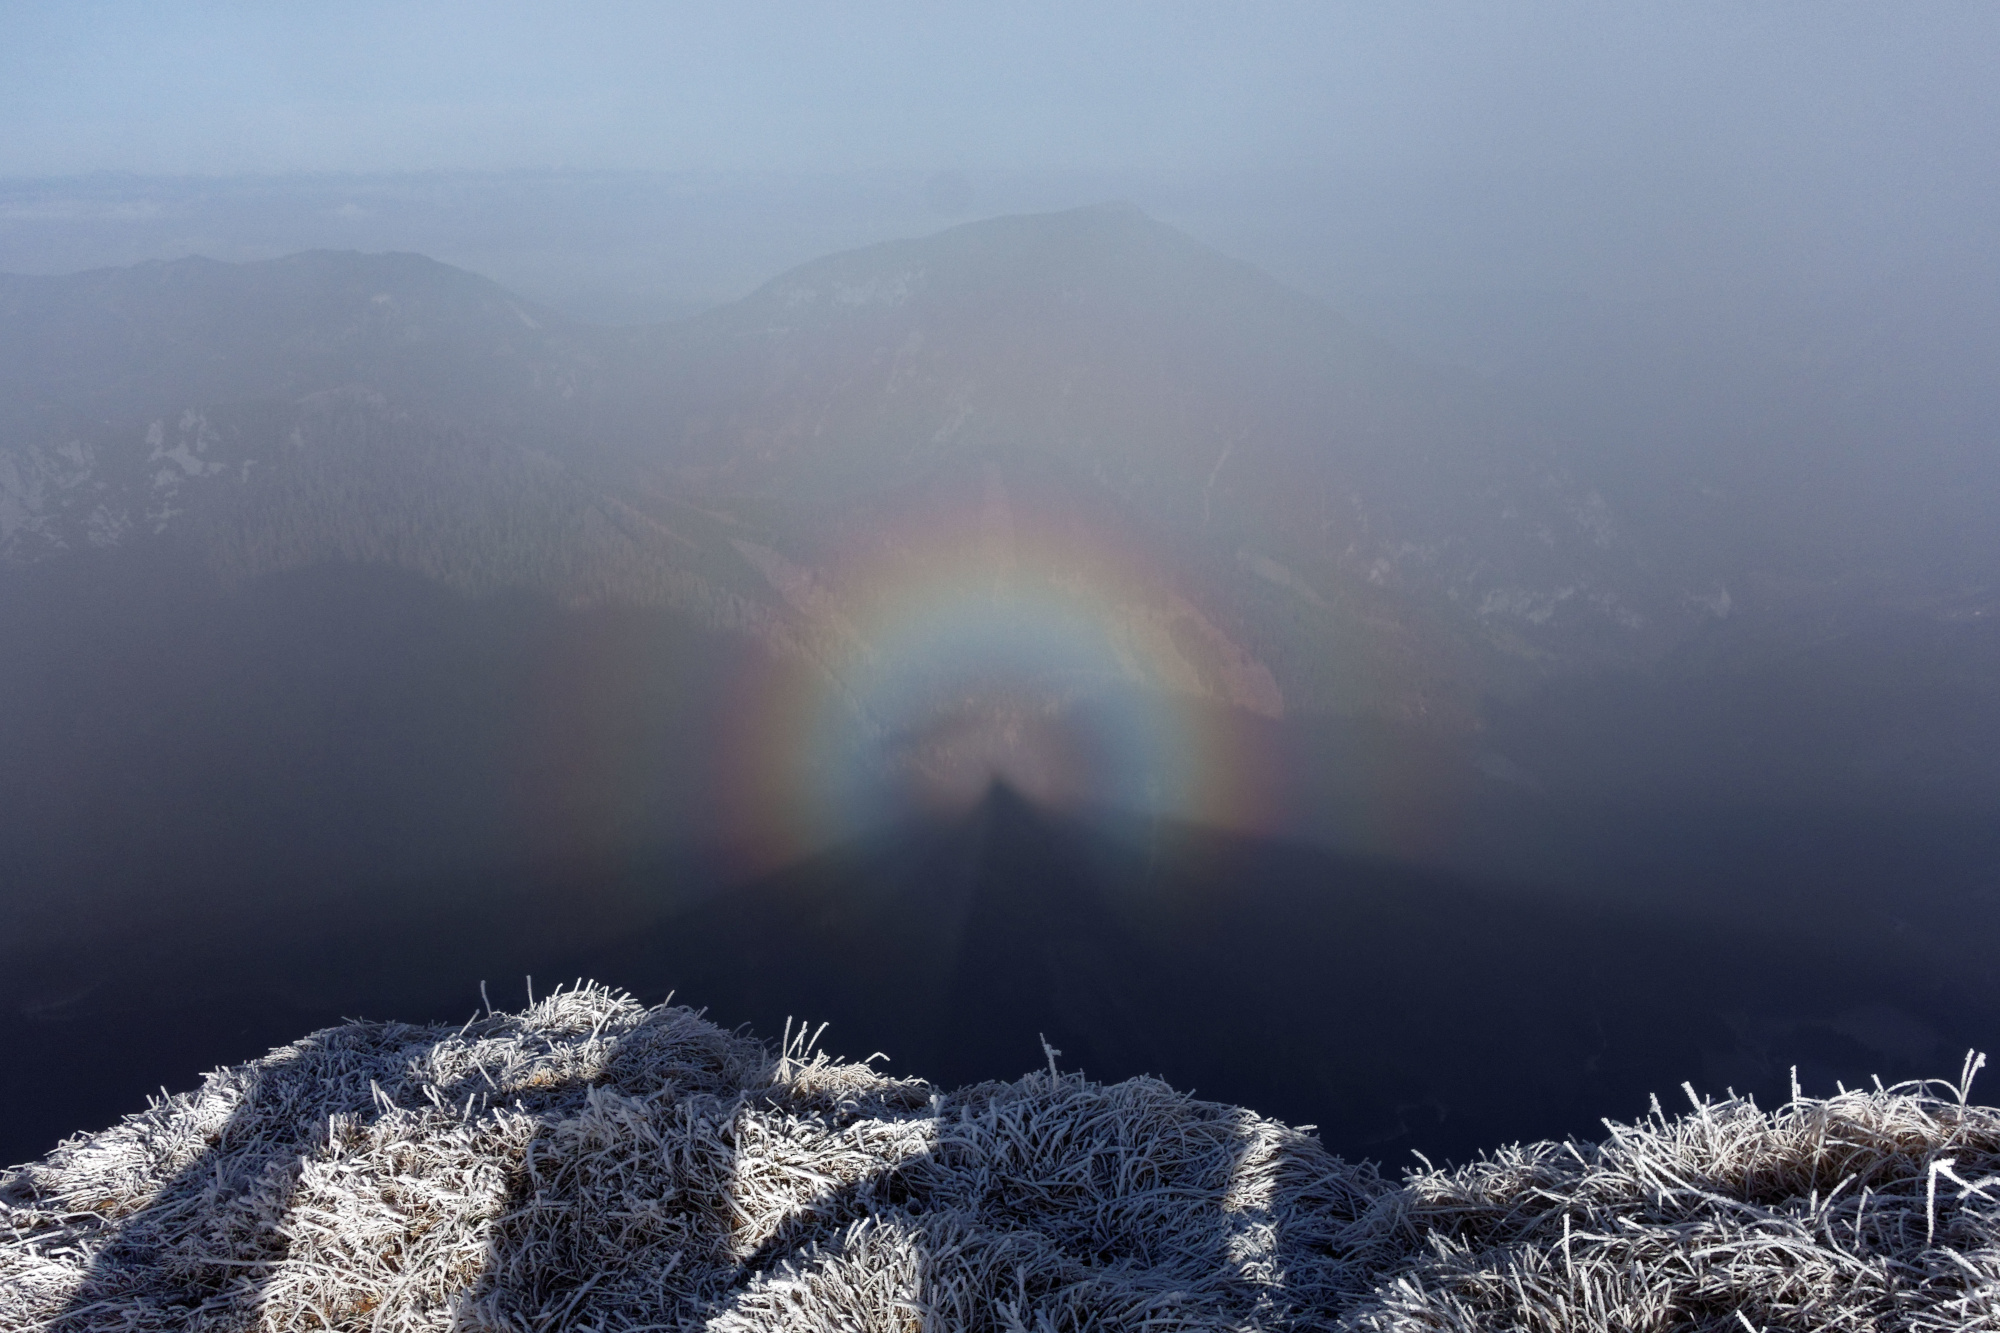
\includegraphics[width=9truecm]{slike/07_Glorija.jpg}\index{Glorija}
\caption{Miejevo sipanje na drobnih kapljicah vode je vzrok za nastanek tako imenovane
glorije. To je pojav, pri katerem so okoli sence opazovalca na megli ali oblaku vidne
barvne ojačitve. Ker je kotna porazdelitev sipanja odvisna od valovne dolžine svetlobe, so
krogi okoli sence videti različnih barv. Iz lege ojačitev lahko ocenimo velikost kapljic, na
prikazanem primeru so kapljice megle velike okoli $7~\si{\micron}$. Foto: Martin Čopič.}
\label{fig:07_Glorija}
\vglue-5truemm
\end{figure}

\begin{remark}
Pri obravnavi sipanja svetlobe smo se omejili le na elastično sipanje, pri katerem se valovna 
dolžina svetlobe ohranja. Poleg tega poznamo neelastično sipanje,\index{Sipanje!{neelastično}}
pri katerem se valovna dolžina\index{Sipanje!{Ramanovo}}\index{Ramanovo sipanje}
sipane svetlobe razlikuje od valovne dolžine vpadne svetlobe. Primer neelastičnega sipanja
je Ramanovo sipanje. Ko se svetloba siplje, se del energije vpadnega valovanja porabi za 
vzbujanje nihanj ali rotacije gradnikov snovi, sipana svetloba pa ima praviloma nižjo frekvenco oziroma
večjo valovno dolžino. Razlika frekvenc vpadne in sipane svetlobe sovpada z energijskimi
nivoji v snovi, zato je Ramanovo sipanje zelo uporabno za spektroskopske metode analize snovi.

Drugi primer neelastičnega sipanja je Brillouinovo sipanje, pri katerem del 
energije\index{Brillouinovo sipanje}\index{Sipanje!{Brillouinovo}}
vpadne svetlobe preide na mrežna nihanja v snovi. Z merjenjem spremembe frekvence sipane svetlobe
glede na frekvenco vpadne svetlobe lahko določimo lastnosti snovi.
\end{remark}
